\chapter{Construção de espaços de probabilidade}

Nessa seção descreveremos diversas maneiras diferentes de construir um espaço de probabilidade, dando diversos exemplos de como elas podem ser usadas na modelagem de diferentes processos reais.

\section{Caso enumerável}

Quando $\Omega$ é finito ou enumerável, tipicamente definimos sobre $\Omega$ a $\sigma$-álgebra das partes, ou seja $\mathcal{F} = \mathcal{P}(\Omega) = \sigma(\{\omega\}_{\omega \in \Omega})$.
Além disso podemos definir probabilidades sobre $(\Omega, \mathcal{F})$ de maneira simples tomando $(p_\omega)_{\omega \in \Omega}$ tais que
\begin{enumerate}[\quad a)]
\item $p_\omega \geq 0$ para todo $\omega \in \Omega$ e
\item $\sum_{\omega \in \Omega} p_\omega = 1$.
\end{enumerate}
De fato, nesse caso definimos $P(A) = \sum_{\omega \in A} p_\omega$ que claramente define uma probabilidade.

\begin{exercise}
  Mostre que se $\Omega$ é finito ou enumerável, toda probabilidade sobre $(\Omega, \mathcal{P}(\Omega))$ é dada como na descrição acima.
\end{exercise}

\begin{example} \mbox{}
  \begin{enumerate}[\quad a)]
  \item Dado $p \in [0,1]$, definimos a medida $\Ber(p)$ \index{distribuicao@distribuição!de Bernoulli} (em homenagem a Bernoulli) em $\{0,1\}$ com $p_1 = p, p_0 = 1-p$.
  \item Dados $n \geq 1$ e $p \in [0,1]$, definimos a medida $\Bin(n,p)$ \index{distribuicao@distribuição!binomial} (binomial) em $\Omega = \{0, 1, \dots, n\}$ com
    \begin{equation}
      p_i = \binom ni p^i (1-p)^{n-i}, \text{ para $i \in \Omega$.}
    \end{equation}
  \item Dado $p \in (0,1]$, em $\Omega = \{0, 1, \dots\}$ definimos a medida $\Geo(p)$ \index{distribuicao@distribuição!geometrica@geométrica} (geométrica) em $\Omega$ induzida pelos pesos
  \begin{equation}
    p_i = (1-p)^i p, \text{ para $i \geq 1$.}
  \end{equation}
  \end{enumerate}
\end{example}

\begin{exercise}
  Seja $\Omega = \{0,1\}^n$ e $p_\omega = \tfrac 1{2^n}$ para todo $\omega \in \Omega$ (ou seja a probabilidade uniforme).
  Considere $X: \Omega \to \{0,1, \dots, n\}$ dada por $X(\omega_1, \dots, \omega_n) = \sum_{i=1}^n \omega_i$.
  Obtenha a distribuição $P_X$.
  Dê um exemplo de medida em $\omega$ para a qual a distribuição de $X$ seja $\Bin(n,p)$.
\end{exercise}

\begin{topics}

\section{Tópico: Método Probabilístico}

Uma importante ferramenta em várias áreas da matemática, tais como Teoria dos Números, Combinatória e Teoria da Computação é o que chamamos de Método Probabilístico. \index{Metodo Probabilistico@Método Probabilístico}

Em várias situações, nós precisamos de mostrar a existência de objetos satisfazendo determinadas propriedades, mas não temos informação suficiente ou capacidade para construí-los explicitamente.
Nesse caso, podemos recorrer ao Método Probabilístico, que simplesmente nos sugere tomar um objeto aleatório de uma maneira esperta e mostrar que com probabilidade positiva as propriedades desejadas serão satisfeitas.
Esse método, apesar de muito ingênuo, é muito eficiente e em diversos casos provê os melhores exemplos conhecidos de certos objetos (para embaraço da comunidade científica).

Nessa seção daremos um exemplo em Teoria dos Números provido primeiramente por Erdõs\footnote{Somos gratos a Robert Morris por sugerir esse teorema como exemplo do Método Probabilístico.}.

\begin{theorem}[Erdös]
  Para todo conjunto finito $A \subset \mathbb{N}$, existe um sub-conjunto $B \subseteq A$ satisfazendo
  \begin{enumerate}[\quad a)]
  \item $\# B \geq \frac{\#A}{3}$ e tal que
  \item não existem $x, y$ e $z \in B$ com $x + y = z$.
  \end{enumerate}
  A propriedade $b)$ acima é o que chamamos de um conjunto ser livre de somas. \index{conjunto!livre de somas}
\end{theorem}

Certamente não temos muita informação sobre $A$, então vamos usar o método probabilístico para a prova desse teorema.

\begin{proof}
  Fixamos $p$ um número primo maior que três vezes o maior elemento de $A$ e considere o espaço $\mathbb{Z}_p$ dos inteiros módulo $p$.
  Seja $X$ um elemento aleatório de $\mathbb{Z}_p$ com distribuição uniforma, isto é $U_{\{0, \dots, p-1\}}$.
  \begin{exercise}
    Mostre que para todo $a \in A$, a multiplicação por $a$ é uma bijeção em $\mathbb{Z}_p$, ou seja
    \begin{equation}
      \mathbb{Z}_p \cdot a = \mathbb{Z}_p.
    \end{equation}
    onde o produto $\mathbb{Z}_p \cdot a$ é entendido elemento a elemento.
    Conclua que
    \begin{equation}
      P \Big[ X \cdot a \in \big[\tfrac p3, \tfrac {2p}3\big) \Big] \geq \frac 13 -\frac 1 p.
    \end{equation}
  \end{exercise}
  Definimos o conjunto aleatório
  $$\mathcal{B} = \{ x\in A \ | X\cdot a \in [\tfrac p3, \tfrac {2p}3) \},$$
  Esse conjunto e livre de soma: se $X=0$ o cojunto e vazio e nos outros casos se $x, y\in \mathcal{B}$
  $$(x+y)\in [\tfrac {2p}3, \tfrac {4p} 3)$$
  que e o complementario de $[\tfrac p3, \tfrac {2p}3)$ em $\mathbb{Z}_p$.

  \medskip

  Basta portanto mostrar que com probabilidade positiva $\# \mathcal{B} \geq \tfrac{\#A}3$, que segue do seguinte argumento.
  \begin{multline*}
    \int \# \mathcal{B} \d P = \int \sum_{a \in A} \1_{\big[ X \cdot a \in [p/3, 2p/3) \big]} \d P \\
    =
    \sum_{a \in A} P \Big[ X \cdot a \in \big[\tfrac p3, \tfrac {2p}3\big) \Big] \geq \frac{\# A}3- \frac{\# A} p> \frac{\# A-1 }3,
  \end{multline*}
  mas para qualquer variável aleatória ,  $P[X \geq \int X \d P] > 0$.
  Nesse caso, isso implica
  $P[X \ge \frac{\# A}3 ]=  P[X > \frac{\# A-1 }3 ]>0$.
\end{proof}

\todo{Adicionar contexto histórico: citar artigo Erdos e o Annals of Math que mostra que não é possível com $\#A(1/3 + \varepsilon)$.}

\end{topics}

\vfill
\pagebreak

\section{Caso absolutamente contínuo}

Uma outra maneira simples de definir um espaço de probabilidade, é partindo de um espaço de medida.
Seja $(\Omega, \mathcal{F}, \mu)$ um espaço de medida e $\rho:\Omega \to \mathbb{R}_+$ uma função mensurável com $\int \rho(x) \mu(\d x) = 1$.
Então podemos definir a probabilidade induzida
\begin{equation}
  \label{e:absolutamente_cont}
  P(A) = \int_A \rho(x) \mu(\d x).
\end{equation}
Nesse caso, chamamos $\rho$ de a \emph{densidade} \index{densidade} de $P$ com respeito a $\mu$.
Uma outra possível notação para a equação acima é $\d P = \rho(x) \d \mu$ \index{dP@$\d P = \rho \d \mu$} (lembrando a derivada de Radon-Nikodim).

Observe que o caso discreto pode ser definido em termos de uma densidade, onde $\rho(\omega) = p_\omega$ e $\mu$ é a medida da contagem em $\Omega$.

\begin{example}
  Vários exemplos podem ser obtidos via \eqref{e:absolutamente_cont} se tomamos $\Omega \subseteq \mathbb{R}$ e $\mu$ a medida de Lebesgue restrita a $\Omega$.
  Nesses casos, escrevemos $P = \rho(x) \d x$ em $\Omega$.
  Alguns exemplos importantes são:
  \begin{enumerate}[\quad a)]
  \item Para $a < b \in \mathbb{R}$, definimos a medida $U[a,b]$ \index{distribuicao@distribuição!uniforme} usando $\rho(x) = \tfrac{1}{b-a}\1_{[a,b]}(x)$.
  \item Para $\lambda > 0$, definimos a medida $\Exp(\lambda)$ \index{distribuicao@distribuição!exponencial} (chamada exponencial de parâmetro $\lambda$) por meio da densidade $\rho(x) = \lambda \exp\{-\lambda x\}$ em $[0,\infty)$.
  \end{enumerate}
\end{example}

Podemos também usar a distribuição de um elemento aleatório para construir outras probabilidades, como mostra o seguinte exemplo.

\begin{example}
  Considere por exemplo $X:[0,2\pi] \to \mathbb{C}$ dada por $X(t) = \exp\{-i t\}$.
  A distribuição imagem $X_*U_{[0,2\pi]}$ é o que chamamos de distribuição uniforme em $\mathbb{S}^1$, também denotada por $U_{S^1}$.
\end{example}

\begin{exercise}
  Mostre que $U_{\mathbb{S}^1}$ não é absolutamente contínua com respeito à medida de Lebesgue em $\mathbb{C} \sim \mathbb{R}^2$.
\end{exercise}

\begin{exercise}
  Mostre que $U_{\mathbb{S}^1}$ é invariante por rotações rígidas de $\mathbb{C}$, isto é, se $T:\mathbb{C} \to \mathbb{C}$ é uma isometria linear,
  $T_*U_{\mathbb{S}^1}=U_{\mathbb{S}^1}$.
\end{exercise}

\begin{exercise}
  Construa uma probabilidade em $S^2$ invariante por rotações.
\end{exercise}

\section{Funções acumuladas de distribuição}

Um caso muito importante de espaço amostral é $\Omega = \mathbb{R}$, principalmente por nos ajudar a entender distribuições de variáveis aleatórias.
Para tanto, precisaremos de uma boa ferramenta para descrever probabilidades em $\mathbb{R}$.

\begin{definition}
  Dada $P$ em $\mathbb{R}$, definimos $F_P:\mathbb{R} \to [0,1]$ por $F_P(x) = P\big((-\infty, x]\big)$.
  Essa função é chamada a \emph{função de distribuição} acumulada de $P$. \index{funcao de distribuicao@função de distribuição}
\end{definition}

\begin{notation}
  Se $X:\Omega \to \mathbb{R}$ é uma variável aleatória num espaço $(\Omega, \mathcal{F}, P)$, denotamos por $F_X$ \index{FX@$F_X$}
  a função de distribuição acumulada correspondente à distribuição $X_*P$.
\end{notation}

Lembramos que uma probabilidade em $\mathbb{R}$ é uma função $P:\mathcal{B}(\mathbb{R}) \to [0,1]$ e o domínio dessa função é bastante complicado.
Por exemplo se quisermos representar uma distribuição de uma variável aleatória no computador através dessa função $P$, teríamos problemas.
Contudo, a função $F_P$ (ou $F_X$) é muito mais simples de ser compreendida ou representada, por seu domínio ser $\mathbb{R}$.

\begin{example}
  Não é difícil verificar que
  \begin{equation}
    F_{\delta_{x_0}} =
    \begin{cases}
      0 & \text{ se $x < x_0$,}\\
      1 & \text{ se $x \geq x_0$}
    \end{cases}
  \end{equation}
  e que
  \begin{equation}
    F_{U_{[0,1]}} =
    \begin{cases}
      0 & \text{ se $x \leq 0$,}\\
      x & \text{ se $x \in [0,1]$ e}\\
      1 & \text{ se $x \geq 1$.}
    \end{cases}
  \end{equation}
\end{example}

\begin{exercise}
  Calcule $F_{\Exp(\lambda)}$.
\end{exercise}

\begin{proposition}
  \label{p:propried_F}
  $F_P$ (e obviamente $F_X$) satisfazem:
  \begin{enumerate}[\quad a)]
  \item $\smash{\lim\limits_{x \to -\infty}} F(x) = 0$, $\smash{\lim\limits_{x \to \infty}} F(x) = 1$,
  \item $F$ é monótona não-decrescente e
  \item $F$ é contínua à direita e possui limite à esquerda (càdlàg, do francês). \index{cadlag@càdlàg}
  \end{enumerate}
\end{proposition}

\begin{proof}
  \begin{enumerate}[\quad a)]
  \item Se $x_n \to -\infty$ monotonamente, então $A_n = (-\infty, x_n]$ são encaixados e de interseção vazia.
    Logo, pela Proposição~\ref{p:prob_continua}, temos $P(A_n) \to 0$.
    O outro caso é análogo.
  \item Se $x \leq x'$ então $(-\infty, x] \subseteq (-\infty,x']$, donde $F(x) \leq F(x')$.
  \item Continuidade à direita (càd) - Se $x_n \downarrow x$ monotonamente, então $A_n = (-\infty, x_n] \downarrow (-\infty, x]$ (eles são encaixados).
    Logo $F(x_n) \to F(x)$.

    Limite à esquerda (làg) - Segue do fato de $F$ ser monótona e limitada. \qedhere
  \end{enumerate}
\end{proof}

\begin{theorem}
  \label{t:existe_prob_R}
  Se $F$ satisfaz as três propriedades listadas na Proposição~\ref{p:propried_F}, então existe uma única $P$ em $(\mathbb{R}, \mathcal{B}(\mathbb{R}))$ tal que $F = F_P$.
\end{theorem}

Poderíamos usar o Teorema da Extensão de Caratheodory para provar tal resultado, de maneira similar ao que foi feito no caso da Medida de Lebesgue.
Mas escolhemos abaixo um método mais simples, que parte da existência de $U_{[0,1]}$.

\begin{proof}
  A unicidade de tal $P$ segue da Proposição~\ref{p:P12_equal_pi} (consequêcia do Teorema de Dynkin), pois se $P$ e $P'$ são tais que $F_{P} = F_{P'}$, então temos que $P\big( (-\infty, x] \big) = P'\big( (-\infty, x] \big)$.
  Mas a classe de intervalos semi-infinitos da forma $(-\infty, x]$ forma um $\pi$-sistema que gera a $\sigma$-álgebra dos borelianos, logo $P = P'$.

  Para construir uma $P$ tal que $F_P = F$, definiremos $S:(0,1) \to \mathbb{R}$, a inversa generalizada de $F$, por
  \begin{equation}
    S(u) = \sup \{x \in \mathbb{R} \, : \,  F(x) < u\}.
  \end{equation}
  \begin{figure}[tb]
    \centering
    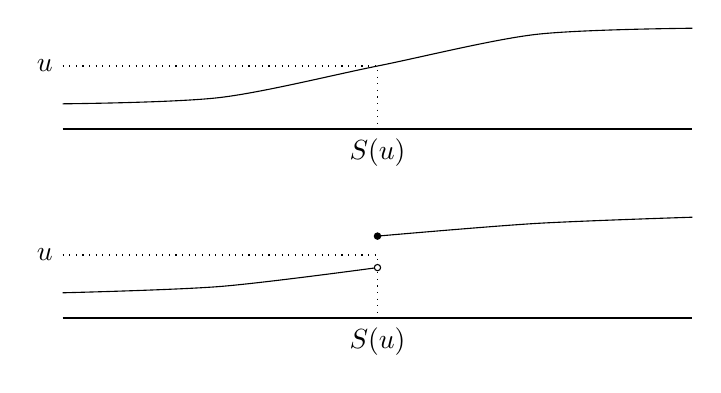
\begin{tikzpicture}[scale=.8]
      \draw (0,1) -- (10,1);
      \draw (0,4) -- (10,4); % second line
      \draw plot [smooth,tension=.5] coordinates{(0, 4.4) (2.5, 4.5) (5,5) (7.5, 5.5) (10, 5.6)};
      \draw plot [smooth,tension=.5] coordinates{(0, 1.4) (2.5, 1.5) (5,1.8)};
      \draw plot [smooth,tension=.5] coordinates{(5, 2.3) (7.5, 2.5) (10,2.6)};
      \draw[dotted] (0,5) -- (5,5) -- (5,4);
      \draw[dotted] (0,2) -- (5,2) -- (5,1);
      \draw [fill,color=white] (5,1.8) circle [radius=0.05];
      \draw (5,1.8) circle [radius=0.05];
      \draw [fill] (5,2.3) circle [radius=0.05];
      \node at (0,5) [left]{$u$};
      \node at (0,2) [left]{$u$};
      \node at (5,1) [below]{$S(u)$};
      \node at (5,4) [below]{$S(u)$};
    \end{tikzpicture}
    \caption{\small Ilustração da definição de $S(u)$.}
    \label{f:Rk_good}
  \end{figure}

  Seja $P = S_* U_{[0,1]}$, isto é $P(A) = U_{[0,1]}(S^{-1}(A))$ e mostraremos que $F_P = F$.
  Para tanto, basta ver que
  \begin{equation}
    \label{e:pseudo_inversa}
    \{u \in [0,1] \, : \,  S(u) \leq x\} = \{u \in [0,1] \, : \,  u \leq F(x)\}, \text{ para todo $x \in \mathbb{R}$}.
  \end{equation}
  Pois isso implicaria que $F_P(x) = U_{[0,1]}[S(u) \leq x] = U_{[0,1]} [u \leq F(x)] = F(x)$.

  Vamos agora checar \eqref{e:pseudo_inversa} observando que:
  \begin{enumerate}[\quad a)]
  \item Se $u \leq F(x)$ então todo $x'$ tal que $F(x') < u$ é menor que $x$.
    Logo $S(u) \leq x$.
  \item Por outro lado, se $x \ge S(u)$ então todo $x' > x$ satisfaz $F(x') > u$.
    Pois por continuidade a direita $F(x)\ge u$.
  \end{enumerate}
  Isos prova \eqref{e:pseudo_inversa}, terminando a prova da proposição.
\end{proof}

\begin{exercise}
  Mostre o resultado acima usando o Teorema de Extensão de Caratheodory.
\end{exercise}

\section{Espaços produto finito}

Dados espaços $\Omega_1, \dots, \Omega_n$ com suas respectivas $\sigma$-álgebras $\mathcal{F}_1, \dots, \mathcal{F}_n$, podemos definir o espaço mensurável produto $(\widebar{\Omega}, \widebar{\mathcal{F}})$ da seguinte forma
\begin{equation}
  \widebar{\Omega} = \prod_{i=1}^n \Omega_i \quad \text{e} \quad \widebar{\mathcal{F}} = \sigma \Big( \{
  A_1 \times \cdots \times A_n  \, : \,  \forall i \in \{1,\dots,n\},\ A_i \in \mathcal{F}_i \} \Big).
\end{equation}
Essa $\sigma$-álgebra e chamada de $\sigma$-álgebra produto e denotaremos ela por $\bigotimes_{i=1}^n \mathcal{F}_i$,
o $\mathcal{F}_1\otimes \mathcal{F}_2$ quando $n=2$.

\begin{proposition}
  Se $(\Omega_1, \mathcal{F}_1, P_1), \dots, (\Omega_n, \mathcal{F}_n, P_n)$ são espaços de probabilidade, então existe uma única probabilidade $\widebar{P}$ no espaço mensurável $(\widebar{\Omega}, \widebar{\mathcal{F}})$ tal que
  \begin{equation}
    \widebar{P}(A_1 \times \cdots \times A_n) = \prod_{i=1}^n P_i(A_i), \text{ para todos $A_i \in \mathcal{F}_i$, $i \leq n$.}
  \end{equation}
  Essa probabilidade é chamada probabilidade produto.
  Usaremos a notação $\bigotimes_{i=1}^n P_i$ o $P_1\otimes P_2 \otimes \dots \otimes P_n$.
\end{proposition}

\begin{proof}
  Teoria da Medida.
\end{proof}

Note que a unicidade do produto pode ser concluída por exemplo usando o Corolário~\ref{c:produto_e_unico}.

\begin{exercise}
  Mostre que o produto de $n$ cópias de $(\{0,1\}, \mathcal{P}(\{0,1\}), \Ber(1/2))$ é a distribuição uniforme em $\{0,1\}^n$.
\end{exercise}

\section{Independência}

Nossa intuição nos diz que quando jogamos duas moedas, o resultado de cada uma delas não deve depender um do outro.
Dessa forma, a probabilidade de obtermos um determinado resultado (como por exemplo duas caras) deve ser um quarto, ou seja meio vezes meio.

Em geral, definimos dois eventos como independentes da seguinte forma.

\begin{definition}
  Dizemos que dois eventos $A, B \in \mathcal{F}$, são \emph{independentes} \index{independencia@independência!de eventos} se
  \begin{equation}
    P(A \cap B) = P(A) P(B).
  \end{equation}
\end{definition}

\begin{example}
  Se $\Omega = \{1, \dots, 6\}$ é dotada da $\sigma$-álgebra das partes e e $P(A) = \#A/6$, então os eventos $A = [\omega \text{ é impar}]$ e $B = [\omega \geq 5]$ satisfazem
  \begin{equation}
    P(A \cap B) = P(\{5\}) = 1/6 = (1/2) (1/3) = P(A) P(B).
  \end{equation}
  Logo tais eventos são independentes.
\end{example}

\begin{exercise}
  Seja $\Omega = \{0,1\}^n$ com $P(A) = \#A/2^n$ e $X_i(\omega_1, \dots, \omega_n) = \omega_i$ para $i = 1, \dots, n$.
  Mostre que
  \begin{equation}
    P[X_i = a, X_j = b] = P[X_i = a] P[X_j = b],
  \end{equation}
  onde $[A, B]$ denota a interseção $[A] \cap [B]$.
\end{exercise}

\subsection{Coleções de eventos}

\todo{discutir a alternativa $I = \{1,\dots, k\}$ que é ruim (basta adicionar $\varnothing$ que qq coisa fica indep).}

\begin{definition}
  Sejam $A_1, A_2, \dots, A_k$ eventos.
  Dizemos que eles formam uma coleção independente \index{independencia@independência!de eventos} se para todo $I \subseteq \{1, \dots, k\}$ não vazio
  \begin{equation}
    P\big( \mcap\nolimits_{i \in I} A_i \big) =  \prod\limits_{i \in I} P(A_i).
  \end{equation}
\end{definition}

Vale observar que independência dois a dois não implica independência.
Mais precisamente
\begin{example}
  Seja $\Omega = \{1,2,3,4\}$ com $P(A) = \# A/4$ e sejam os seguintes eventos: $A_1 = \{1,2\}$, $A_2 = \{2,3\}$ e $A_3 = \{1,3\}$.
  Nesse caso,
  \begin{enumerate}[\quad a)]
  \item $P(A_i) = 1/2$ para $i = 1, 2, 3$,
  \item $P(A_i \cap A_j) = 1/4$ para todo $i \neq j$ mas
  \item $P(A_1 \cap A_2 \cap A_3) = 0 \neq 1/8 = P(A_1) P(A_2) P(A_3)$.
  \end{enumerate}
\end{example}

\begin{definition}
  Dizemos que uma coleção infinita de eventos $(A_n)_{n\ge 1}$ é independente \index{independencia@independência!de eventos} se toda sub-coleção finita de tais eventos forem independentes.
\end{definition}

\begin{lemma}
  Se $(A_n)_{n\ge 1}$ forma uma sequencia de eventos independentes, então
  \begin{equation}
    P\Big( \mcap_{i=1}^{\infty} A_i \Big) = \prod\limits_{i=1}^{\infty} P(A_i).
  \end{equation}
\end{lemma}

\begin{proof}
  De fato,
  \begin{equation*}
    P\Big( \mcap_{i=1}^{\infty} A_i \Big) = \lim_{n\to \infty} P\Big( \mcap_{i = 1}^n A_i \Big) = \lim_{n\to \infty} \prod\limits_{i=1}^n P(A_i) = \prod\limits_{i=1}^{\infty} P(A_i). \qedhere
  \end{equation*}
\end{proof}

\begin{exercise}
  Mostre que se $A \in \mathcal{F}$, então $\{B \in \mathcal{F}\, : \, B \text{ é independente de } A\}$ é um $\lambda$-sistema.
\end{exercise}

\begin{exercise}
  Mostre que se $B$ é independente de $A$ para todo $B \in \mathcal{B}$, com $\mathcal{B}$ um $\pi$-sistema, então $B$ é independente de $A$ para todo $B \in \sigma(\mathcal{B})$.
\end{exercise}

\subsection{Independência de \texorpdfstring{$\sigma$}{sigma}-álgebras}

\begin{definition}
  Dado um espaço de probabilidade $(\Omega,P,\mathcal{F})$ Dizemos que as $\sigma$-álgebra $\mathcal{F}_1,\dots,\mathcal{F}_n\subset \mathcal{F}$ são independentes \index{independencia@independência!de sigma-algebras@de $\sigma$-álgebras} se
  \begin{equation}
    \forall \mathcal{A}_1\in \mathcal{F}_1,\dots ,\mathcal{A}_n \in \mathcal{F}_n, \ P(\cap_{i=1}^n A_i)=\prod_{i=1}^n P(A_i).
  \end{equation}
  Nessa definição podemos tomar uma coleção infinita.
\end{definition}

\begin{exercise}
  Em um espaço produto $(\Omega_1 \times \Omega_2, \mathcal{F}_1 \otimes \mathcal{F}_2, P_1 \otimes P_2)$, podemos definir
  \begin{equation}
    \begin{split}
      \widebar{\mathcal{F}}_1 & = \{A \times \Omega_2 \, : \, A \in \mathcal{F}_1\},\\
      \widebar{\mathcal{F}}_2 & = \{\Omega_1 \times B \, : \, B \in \mathcal{F}_2\}.
    \end{split}
  \end{equation}
  Mostre que essas $\sigma$-álgebras são independentes.
\end{exercise}

Podemos extender esse conceito a elementos aleatórios, ou seja:
\begin{definition}
  Dizemos que $X_1, \dots, X_k$ são elementos aleatórios independentes \index{independencia@independência!de elementos} se as respectivas $\sigma$-álgebras $\sigma(X_1), \dots, \sigma(X_k)$ o forem.
\end{definition}

Quando $X_1, \dots, X_k$ são elementos aleatórios independentes e com a mesma distribuição, escrevemos que $X_i$ são \iid (independentes e identicamente distribuídos).

\begin{exercise}
  Com a notação do exercício anterior, mostre que as funções $X_i:\Omega_1 \times \Omega_2 \to \Omega_i$ dadas por
  \begin{equation}
    X_1(x,y) = x \text{ e } X_2 (x,y) = y,
  \end{equation}
  são elementos aleatórios e são independentes.
\end{exercise}

\begin{exercise}
  Mostre que as coordenadas canônicas do exercício anterior no caso $X_i: \mathbb{R}^2 \to \mathbb{R}$ não são independentes segundo a medida $U_{\mathbb{S}^1}$.
  Mas o são segundo $U_{[0,1]^2}$ (que é a medida de Lebesgue em $\mathbb{R}^2$ restrita a $[0,1]^2$).
\end{exercise}

\begin{exercise}
  Seja $\Omega = \{0,1\}^n$ com $P(A) = \#A/2^n$ e $X_i(\omega_1, \dots, \omega_n) = \omega_i$ para $i = 1, \dots, n$.
  Mostre que os $X_i$ são independentes.
\end{exercise}

\begin{exercise}
  Sejam $(X_i)_{i \geq 1}$ elementos aleatórios independentes tomando valores em espaços $(E_i)_{i \geq 1}$, respectivamente.
  Mostre que para funções mensuráveis $(f_i)_{i \geq 1}$ temos que $(f_i(X_i))_{i \geq 1}$ são independentes.
\end{exercise}

\begin{exercise}
  Mostre que se $X, Y$ são elementos aleatórios e se $X$ é constante quase certamente então $X$ e $Y$ são independentes.
\end{exercise}

\begin{exercise}
  Sejam $X$ e $Y$ variáveis aleatórias independentes com distribuição $\Exp(1)$, calcule a distribuição de
  \begin{enumerate}[\quad a)]
  \item $\min\{X,Y\}$ e
  \item $X + Y$.
  \end{enumerate}
\end{exercise}

\begin{exercise}
  Seja um espaço produto de medidas $(\Omega_1 \times \Omega_2, \mathcal{F}_1 \otimes \mathcal{F}_2, \mu_1 \otimes \mu_2)$ e defina a probabilidade $P$ através de
  \begin{equation}
    \d P = \rho(x,y) \d (\mu_1 \otimes \mu_2).
  \end{equation}
  Mostre nesse caso que as coordenadas canônicas $X_1$ e $X_2$ são independentes se e somente se existem $\rho_1$ e $\rho_2$ em $\Omega_1$ e $\Omega_2$ respectivamente, tais que $\rho(x,y) = \rho_1(x) \rho_2(y)$ quase certamente com respeito a $\mu_1 \otimes \mu_2$.
\end{exercise}

\begin{exercise}
  Sejam $X, Y$ vari\'aveis aleat\'orias tais que
  \begin{equation}
    P[X \leq x, Y \leq y] =
    \begin{cases}
      0 & \quad \text{if $x < 0$,}\\
      (1-e^{-x}) \Big(\frac 12 + \frac 1\pi \tan^{-1} y \Big), & \quad \text{if $x \geq 0$}.
    \end{cases}
  \end{equation}
  \begin{enumerate}[\quad a)]
  \item Mostre que a distribui\c{c}\~ao conjunta $\mu_{(X,Y)}$ \'e
    absolutamente cont\'inua com rela\c{c}\~ao \`a medida de Lebesgue em
    $\mathbb{R}^2$.
  \item Mostre que $X$ e $Y$ s\~ao independentes.
  \end{enumerate}
\end{exercise}

\begin{exercise}
  \label{x:convolucao_densidade}
  Mostre que se $X, Y$ são variáveis aleatórias independentes com distribuições $X \distr f_X(x) \d x$ e $Y \distr f_Y(y) \d y$, então $X + Y$ tem distribuição absolutamente contínua com respeito a Lebesgue e
  \begin{equation}
    f_{X + Y}(z) = \int_{-\infty}^\infty f_Y(z - x) f_X(x) \d x.
  \end{equation}
\end{exercise}

\todo{mandar para depois de produtos infinitos?}

\begin{lemma}[Borel-Cantelli - segunda parte]
  Se $A_1, A_2, \dots \in \mathcal{F}$ são independentes e $p_i = P(A_i)$ satisfazem $\sum_i p_i = \infty$, então
  \begin{equation}
    P[A_i \text{ infinitas vezes}] = 1.
  \end{equation}
\end{lemma}

\begin{proof}
  Queremos mostrar que
  \begin{equation}
    P \Big( \big(\mcap_n \mcup_{i=n}^\infty A_i\big)^c \Big) = 0,
  \end{equation}
  mas
  \begin{equation}
    P \Big( \big(\mcap_n \mcup_{i=n}^\infty A_i\big)^c \Big) = P \Big(\mcup_n \mcap_{i=n}^\infty A_i^c \Big) \leq \sum\limits_n P \Big(\mcap_{i=n}^\infty A_i^c \Big).
  \end{equation}
  Logo basta mostrar que a probabilidade à direita é zero para todo $n$.
  Mas
  \begin{equation}
    \begin{split}
      P \Big(\mcap_{i=n}^\infty A_i^c \Big) & = \prod\limits_{i=n}^\infty P(A_i^c) = \prod\limits_{i=n}^\infty (1 - p_i)\\
      & \leq \prod\limits_{i=n}^\infty \exp\{-p_i\} = \exp\big\{- \sum_{i=n}^\infty p_i\big\} = 0.
    \end{split}
  \end{equation}
  Terminando a prova do lemma.
\end{proof}

\todosec{Tópico: Uma dinâmica em \texorpdfstring{$[0,1]$}{[0,1]}}{fazer dinâmica 2x mod 1 e relações Lebesgue[0,1] com produtos de bernoulli}

\begin{topics}

\section{Tópico: Lei dos pequenos números}

Nessa seção estudaremos como se comportam limites de algumas variáveis aleatórias bastante importantes, mas primeiramente, uma breve intuição.

Apesar de que descreveremos a nossa motivação a partir desse exemplo do estudo de um material radioativo, podemos encontrar aplicações com justificativas bastante semelhantes para outros problemas, como: chegada de carros em um sinal de trânsito, número de mutações em um gene, número de mortes por ano em uma faixa etária...

Digamos que estamos observando um material radioativo que esporadicamente emite fótons que podemos detectar através de um aparelho.
A razão dessas emissões pode ser aproximada pelo seguinte modelo.
Na amostra temos um número $n$ grande de átomos instáveis ($n \sim 10^{23}$) e em um determinado tempo de observação, cada um deles tem probabilidade muito baixa de decair emitindo um fóton (digamos $p \sim 10^{-23}$).
Nesse caso, supondo que todos decidam emitir de maneira independente, temos para $p \in [0,1]$,
\begin{equation}
  \label{e:Poisson_setup}
  \Omega_n = \{0,1\}^n, \quad \mathcal{F}_n = \mathcal{P}(\Omega) \quad \text{e} \quad P_p = \otimes_{i=1}^n Ber(p).
\end{equation}
Dessa forma, o número total de emissões observadas para $\omega = (\omega_1, \dots, \omega_n) \in \Omega$ é
\begin{equation}
  \label{e:Xn_Poisson}
  X_n(\omega) = \sum_{i=1}^n \omega_i.
\end{equation}
E gostaríamos de entender como se comporta essa distribuição, que nada mais é que $\Bin(n,p)$.

Uma primeira tentativa seria modelar esse processo dizendo que o número de átomos $n$ é tão grande, que somente estamos interessados no comportamento assimtótico quando $n$ vai para infinito.
Mas para manter o número de emissões sob controle, também gostaríamos que $p = p_n$, que converge a zero.
Poderíamos por exemplo escolher
\begin{equation}
  p_n = \frac \lambda n.
\end{equation}
Mas a discussão que se segue é muito mais geral que essa escolha específica.

Como estaremos interessados em um regime assimtótico da distribuição de $X_p$ (lembre que apesar do espaço amostral de $X_n$ variar com $n$, sua distribuição é sempre uma probabilidade em $\mathbb{N}$).
Mas para falar de regimes assimtóticos, precisamos de definir uma noção de distância entre duas distribuições em $\mathbb{N}$.

\begin{definition}
Dadas duas distribuições $\mu_1$ e $\mu_2$ em $(\Omega, \mathcal{A})$, definimos
\begin{equation}
  \lVert \mu_1 - \mu_2 \rVert_{\VT} = \sup_{A \in \mathcal{A}} |\mu_1(A) - \mu_2(A)|,
\end{equation}
\index{mu1 - mu2@$\lVert \mu_1 - \mu_2 \rVert$} chamada de distância em variação total \index{variacao total@variação total} entre $\mu_1$ e $\mu_2$.
\end{definition}

No nosso caso, $\Omega$ é enumerável.
Vamos ver que nesse caso é possível reescrever a definição acima de modo a ver mais facilmente que se trata de uma distância no espaço de probabilidades em $\Omega$.

\begin{lemma}
  \label{l:vt_l1}
  Se $\Omega$ for finito ou enumerável, então podemos escrever
  \begin{equation}
    \lVert \mu_1 - \mu_2 \rVert_{\VT} = \frac{1}{2} \sum_{x \in \Omega} |\mu_1(x) - \mu_2(x)|.
  \end{equation}
\end{lemma}

\begin{proof}
Para mostrar que o lado esquerdo é maior ou igual ao direito, escolhemos $A = \{ x \in \Omega \, : \, \mu_2(x) \leq \mu_1(x)\}$. Assim
\begin{equation}
  \begin{split}
    \sum_{x \in A} \mu_1(x) - \mu_2(x) & = |\mu_1(A) - \mu_2(A)|\\
    & = |\mu_1(A^c) - \mu_2(A^c)| = \sum_{x \in A^c} \mu_2(x) - \mu_1(x),
  \end{split}
\end{equation}
donde
\begin{equation}
  \lVert \mu_1 - \mu_2 \rVert_{\VT} \geq |\mu_1(A) - \mu_2(A)| = \frac{1}{2} \sum_{i} |\mu_1(x_i) - \mu_2(x_i)|.
\end{equation}

Na outra direção, observe que para todo $B \subseteq \Omega$,
\begin{equation}
  \begin{split}
    \sum_{i} |\mu_1(x_i) - \mu_2(x_i)| & \geq \sum_{x \in B} \mu_1(x) - \mu_2(x) + \sum_{x \in B^c} \mu_1(x) - \mu_2(x)\\
    & = \mu_1(B) - \mu_2(B) + (1 - \mu_2(B)) - (1 - \mu_1(B))\\
    & = 2(\mu_1(B) - \mu_2(B)).
  \end{split}
\end{equation}
O que termina a prova do lema.
\end{proof}

Fica agora claro que $\lVert \mu_1 - \mu_2 \rVert_{\VT}$ determina uma distância.

\begin{exercise}
Mostre um lema análogo ao anterior para $(\Omega, \mathcal{A})$ qualquer, desde que $\mu_1$ e $\mu_2$ sejam absolutamente contínuas com relação à uma medida fixa nesse espaço mensurável. Nesse caso utilizaremos as derivadas de Radon–Nikodym.
\end{exercise}

Como estaremos interessados em variáveis independentes, precisamos de um resultado que relacione a distância em variação total com produtos de medida. Isso é parte do seguinte

\begin{lemma}
\label{l:vt_produto}
Sejam $\mu_1, \mu_2$ distribuições em $\Omega$ e $\nu_1, \nu_2$ distribuições em $\Omega'$ ambos enumeráveis. Então
\begin{equation}
  \lVert \mu_1 \otimes \nu_1 - \mu_2 \otimes \nu_2 \rVert_{\VT} \leq \lVert \mu_1 - \mu_2 \rVert_{\VT} + \lVert \nu_1 - \nu_2 \rVert_{\VT}.
\end{equation}
\end{lemma}

\begin{proof}
Basta expandir
\begin{equation}
  \begin{split}
    2\lVert \mu_1 & \otimes \nu_1 - \mu_2 \otimes \nu_2 \rVert_{\VT} = \sum_{x \in \Omega, y \in \Omega'} |\mu_1(x)\nu_1(y) - \mu_2(x)\nu_2(y)|\\
    & \leq \sum_{x \in \Omega, y \in \Omega'} |\mu_1(x)\nu_1(y) - \mu_1(x)\nu_2(y)| + |\mu_1(x)\nu_2(y) - \mu_2(x)\nu_2(y)|\\
    & \leq 2\lVert \mu_1 - \mu_2 \rVert_{\VT} + 2\lVert \nu_1 - \nu_2 \rVert_{\VT}.
  \end{split}
\end{equation}
Onde acima nós usamos que $\mu_1$ e $\nu_2$ são probabilidades. Isso termina a prova do lema.
\end{proof}

Finalmente, gostaríamos de entender como a distância de variação total se comporta com respeito à soma de variáveis independentes.
Isso estará ligado à convolução de distribuições:

\begin{definition}
Dadas, $\mu$ e $\nu$ distribuições em $\mathbb{Z}$, definimos a distribuição
\begin{equation}
  (\mu \star \nu)(x) := \sum_{y \in \mathbb{Z}} \mu(x-y) \nu(y).
\end{equation}
\end{definition}

Essa definição se relaciona com a soma de variáveis independentes graças ao seguinte
\begin{exercise}
Se $X \overset{d}\sim \mu$ e $Y \overset{d}\sim \nu$ são variáveis aleatórias inteiras e independentes, então $X + Y \overset{d}\sim \mu \star \nu$.
Dica: particione o espaço amostral nos eventos $[X = j]$, para $j \in \mathbb{Z}$, como na prova do Lema~\ref{l:soma_poisson} abaixo.
\end{exercise}

\begin{corollary}
Se $\mu$ e $\nu$ são distribuições em $\mathbb{Z}$, então $\mu \star \nu = \nu \star \mu$.
\end{corollary}

Como prometido, obtemos a seguinte relação entre a convolução e a distância de  variação total.
\begin{lemma}
\label{l:vt_conv}
Sejam $\mu$, $\nu$ duas medidas em $\Omega$ enumerável e $X:\  (\Omega,\mathcal{P}(\Omega))\to (E,\mathcal{A})$ um elemento aleatorio
\begin{equation}
   \lVert X_*\mu - X_*\nu\rVert_{\VT}\le    \lVert \mu - \nu\rVert_{\VT}.
\end{equation}
Em particular se $\mu_1, \mu_2, \nu_1, \nu_2$ são distribuições em $\mathbb{Z}$, então
\begin{equation}
  \lVert \mu_1 \star \nu_1 - \mu_2 \star \nu_2 \rVert_{\VT} \leq \lVert \mu_1 \otimes \nu_1 - \mu_2 \otimes \nu_2 \rVert_{\VT}
\end{equation}
\end{lemma}

\begin{proof}
O segundo ponto segue do primeiro applicado ao caso $\Omega = \mathbb{Z}^2$, $E=\mathbb{Z}$ e $X:\ (x,y) \mapsto (x+y)$.
Pelo primeiro, observamos
\begin{equation}
  \begin{split}
    2\lVert X_*\mu - X_*\nu\rVert_{\VT} &= \sum_{x \in X(\Omega)} \Big| \mu(X(\omega)=x) - \nu(X(\omega)=x) \Big|\\
    & =  \sum_{x \in X(\Omega)} \Big| \sum_{\omega \in\Omega \ : \ X(\omega)=x}  \mu(\omega) - \nu(\omega) \Big|\\
    & \leq \sum_{\omega \in \Omega} \big| \mu(\omega)- \nu(\omega) \big|\\
    & = 2\lVert \mu - \nu\rVert_{\VT}.
  \end{split}
\end{equation}
provando o lema.
\end{proof}

Para enunciar o resultado principal dessa seção, vamos apresentar uma distribuição em $\mathbb{N}$ bastane importante, que em particular se comporta muito bem com respeito a somas de variáveis independentes, como veremos.

\begin{definition}
  Uma variável aleatória $X$ é dita ter distribuição de Poisson \index{distribuicao@distribuição!de Poisson} com parâmetro $\lambda$, se
  \begin{equation}
    P[X = k] = \frac{\lambda^k e^{-\lambda}}{k!}, \text{ para $k \geq 0$ inteiro.}
  \end{equation}
  Denotamos isso por $X \overset{d}\sim \Poisson(\lambda)$.
\end{definition}

A distribuição de Poisson se comporta bem com respeito a somas independentes, como mostra o seguinte
\begin{lemma}
\label{l:soma_poisson}
Sejam $X \overset{d}\sim \Poisson(\lambda_1)$ e $Y \overset{d}\sim \Poisson(\lambda_2)$ independentes, então $X+Y \overset{d}\sim \Poisson(\lambda_1 + \lambda_2)$.
\end{lemma}

\begin{proof}
Basta calcular
\begin{equation}
  \begin{split}
    P[X+Y = k] & = \sum_{j = 0}^k P[X = j, Y = k-j] = \sum_{j = 0}^k \frac{\lambda_1^j e^{-\lambda_1} \lambda_2^{k-j} e^{-\lambda_2}}{j! (k-j)!}\\
    & = e^{-(\lambda_1 + \lambda_2)} \frac{1}{k!} \sum_{j = 0}^k \frac{k!}{j! (k-j)!} \lambda_1^j \lambda_2^{k-j} = \frac{e^{(\lambda_1 + \lambda_2)} (\lambda_1 + \lambda_2)^k}{k!},
  \end{split}
\end{equation}
mostrando o resultado.
\end{proof}

Nossa próxima tarefa é estimar a distância entre uma variável aleatória com distribuição $\Ber(p)$ e uma $\Poisson(p)$, como segue.

\begin{lemma}
\index{Lei!dos Pequenos Numeros@dos Pequenos Números}
\label{l:vt_ber_poiss}
Para $p \in [0,1]$, seja $\mu_1 = \Ber(p)$ e $\mu_2 = \Poisson(p)$, então,
\begin{equation}
  \lVert \mu_1 - \mu_2 \rVert_{\VT} \leq p^2.
\end{equation}
\end{lemma}

\begin{proof}
Sabemos que
\begin{equation}
  \begin{split}
    \lVert \mu_1 - \mu_2 \rVert_{\VT} & = \frac{1}{2} \sum_{x} |\mu_1(x) - \mu_2(x)|\\
    & = \frac{1}{2} \Big( |\mu_1(0) - \mu_2(0)| + |\mu_1(1) - \mu_2(1)| + \sum_{x \geq 2} \mu_2(x) \Big)\\
    & = \frac{1}{2} \Big( e^{-p} - (1-p) + p(1-e^{-p}) + (1 - e^{-p} - p e^{-p}) \Big)\\
    & = \frac{2}{2} p (1 - e^{-p}) \leq p^2,
  \end{split}
\end{equation}
terminando a prova.
\end{proof}

O teorema principal de convergência dessa seção concerne a soma de variáveis Bernoulli.

\begin{theorem}[Lei dos Pequenos Números]
  \label{t:lei_peq_numeros}
  Dado, $n \geq 1$ e $p \in [0,1]$, suponha que $\Omega_n$, $\mathcal{F}_n$ e $P_p$ sejam dados como em \eqref{e:Poisson_setup}.
  Então,
  \begin{equation}
    \lVert \Bin(n,p) - \Poisson(pn) \rVert_{\VT} \leq n p^2.
  \end{equation}
\end{theorem}

\begin{proof}
  Basta observar que
  \begin{equation}
    \begin{split}
      \lVert X_n \circ P_p - \Poisson(pn) \rVert_{\VT} & \overset{\text{Lema~\ref{l:soma_poisson}}}= \lVert \Ber(p)^{\star n} - \Poisson(p)^{\star n} \rVert_{\VT}\\
      \overset{\text{Lema~\ref{l:vt_conv}}}\leq & \lVert \Ber(p)^{\otimes n} - \Poisson(p)^{\otimes n} \rVert_{\VT}\\
      \overset{\text{Lema~\ref{l:vt_produto}}}\leq & n \lVert \Ber(p) - \Poisson(p) \rVert_{\VT} \overset{\text{Lema~\ref{l:vt_ber_poiss}}}\leq n p^2,
    \end{split}
  \end{equation}
  provando o teorema.
\end{proof}

\begin{corollary}
  No mesmo contexto do teorema acima, se $p = \lambda/n$, então temos
  \begin{equation}
    \lVert \Bin(n,p) - \Poisson(pn) \rVert_{\VT} \leq \lambda^2 / n,
  \end{equation}
  que converge a zero com $n$.
\end{corollary}
Veremos mais tarde que existem outros tipos de convergência.


\begin{exercise}
  Fixado $\lambda > 0$, seja $N$ uma variável aleatória com distribuição Poisson($\lambda$), isto é
  \begin{equation}
    P[N = k] = \frac{\lambda^k e^{-\lambda}}{k!} \text{ para $k = 0, 1, \dots$}
  \end{equation}
  Considere no mesmo espaço de probabilidade uma sequência de variáveis aleatórias $X_1, X_2, \dots$ que sejam \iid, com distribuição $\Ber(1/2)$ e independentes de $N$.
  \begin{enumerate}[\quad a)]
  \item Calcule a distribuição de $Z = \sum_{i=1}^N X_i$.
  \item Mostre que $Z$ e $N - Z$ são independentes.
  \end{enumerate}
\end{exercise}

\end{topics}

\section{Espaços produto infinito}
\label{s:Omega_produto}

Nessa seção estudaremos $\Omega$ que são dados por produtos enumeráveis de outros espaços de probabilidade.
Mas antes iremos recordar o Teorema da Extensão de Caratheodory.

\subsection{Recordar é viver...}

Vamos lembrar o enunciado do Teorema da Extensão de Caratheodory \index{Teorema!da Extensao de Caratheodory@da Extensão de Caratheodory}.
Antes, vamos relembrar uma definição definição importante.
Uma família $\mathcal{G} \subseteq \mathcal{P}(\Omega)$ é dita uma álgebra de conjuntos \index{anel de conjuntos} se valem:
\begin{enumerate}[\quad a)]
  \item $\Omega \in \mathcal{G}$.
  \item Se $A \in \mathcal{G}$, então $A^c \in \mathcal{G}$.
  \item Para todo $n \geq 1$, se $A_1, \dots, A_n \in \mathcal{G}$, então $\bigcup_{i=1}^n A_i \in \mathcal{G}$.
\end{enumerate}

\begin{theorem}[Teorema da Extensão de Caratheodory]
  Seja $\mathcal{G} \subseteq \mathcal{P}(\Omega)$ uma álgebra de conjuntos em $\Omega$ e suponha que $\mu: \mathcal{G} \to \mathbb{R}_+$ satisfaça a seguinte propriedade:
  \begin{display}
    \label{e:aditiva_na_algebra}
    Se $(A_i)_{i\in I}$ e uma familia finita ou enumerável de elementos disjuntos de $\mathcal G$ tal que $\cup_{i\in I} A_i \in \mathcal{G}$,\\
  temos $\mu(\cup_{i\in I} A_i) = \sum_{i\in I} \mu(A_i)$.
  \end{display}
  Então existe uma medida $\widebar{\mu}: \sigma(\mathcal{G}) \to \mathbb{R}_+$ tal que $\widebar{\mu}(A) = \mu(A)$ para todo $A \in \mathcal{G}$.
\end{theorem}

Mostraremos agora uma consequência simples do teorema acima, que é muito utilizada em probabilidade.

\begin{lemma}[Extensão por continuidade no vazio]
  \label{l:extensao_vazio}
  \index{continuidade no vazio}
  Seja $\mathcal{G} \subseteq \mathcal{P}(\Omega)$ uma álgebra de conjuntos em $\Omega$ e suponha que $P: \mathcal{G} \to \mathbb{R}_+$ satisfaça as seguintes propriedades:
  \begin{enumerate}[\quad a)]
  \item $P(\Omega) = 1$,
    \item $P$ é finitamente aditiva e
    \item sempre que $B_1 \supseteq B_2 \supseteq \dots \in \mathcal{G}$ forem tais que $\cap_i B_i = \varnothing$ (denotamos isso por $B_i \downarrow \varnothing$), temos que $\lim_i \mu(B_i) = 0$.
  \end{enumerate}
  Então existe uma única medida $\widebar{P}: \sigma(\mathcal{G}) \to \mathbb{R}_+$ tal que $\widebar{P}(A) = P(A)$ para $A \in \mathcal{G}$.
\end{lemma}

Observe que $P(\Omega) = 1$ somente é necessário para provar a unicidade de $\widebar{P}$, então poderíamos tentar mostrar uma versão mais geral desse lema.
Mas no contexto de medidas infinitas, não é de se esperar que $B_i \downarrow \varnothing$ implique $\lim_i \mu(B_i) = 0$, como foi assumido acima (veja também a Proposição~\ref{p:prob_continua}).
Portanto resolvemos escrever o enunciado com probabilidades.

\begin{exercise}
  Dê um exemplo de medida que não satisfaz a segunda hipótese do Lema~\ref{l:extensao_vazio}.
\end{exercise}

\begin{proof}
  Primeiro observe que a unicidade segue da Proposição~\ref{p:P12_equal_pi}, já que $\mathcal{G}$ é um $\pi$-sistema.
  Iremos agora mostrar que a propriedade \eqref{e:aditiva_na_algebra} é válida para $P$, logo tome $A_1, A_2, \dots \in \mathcal{G}$ disjuntos e tais que $A = \cup_{i\in \mathbb{N}} A_i \in \mathcal{G}$.
  Definimos o ``resto da união'' por
  \begin{equation}
    B_n = A \setminus \mcup_{i=1}^n A_i.
  \end{equation}
  Claramente
  \begin{enumerate}[\quad a)]
  \item $B_n \downarrow \varnothing$ e
  \item $B_n \in \mathcal{G}$, pois $\mathcal{G}$ é uma álgebra.
  \end{enumerate}

  Logo podemos escrever $A$ como a união disjunta $A = \bigcup_{i=1}^n A_i \cup B_n$ e já que $P$ é finitamente aditiva,
  \begin{equation}
    P(A) = \sum_{i=1}^n P(A_i) + P(B_n),
  \end{equation}
  mas como $\lim_{n\to \infty} P(B_n) = 0$, temos
  \begin{equation}
    P(\cup_{i=1}^{\infty} A_i) = \sum_{i=1}^{\infty} P(A_i),
  \end{equation}
  mostrando a propriedade \eqref{e:aditiva_na_algebra} e concluindo o teorema.
\end{proof}

\subsection{Teorema da Extensão de Kolmogorov}

O objetivo desta seção é provar um resultado que nos permitirá construir probabilidades em espaços produtos infinitos.
Antes precisaremos de introduzir algumas notações.
Dada uma coleção de espaços $(E_i)_{i\in \mathbb{N}}$, definimos o espaço produto
\begin{equation}
  \Omega = \prod_{i=1}^{\infty} E_i = \big\{(\omega_i)_{i\in \mathbb{N}} \, : \,  \omega_i \in E_i \text{ para todo $i \geq 1$}\big\}.
\end{equation}
e os mapas $X_i:\Omega \to E_i$, definidos para $i = 1, 2, \dots$ por
\begin{equation}
  X_i(\omega_1, \omega_2, \dots) = \omega_i,
\end{equation}
que chamamos de \emph{coordenadas canônicas} \index{coordenadas canonicas@coordenadas canônicas} associadas ao produto $\Omega$.

Se cada $E_i$ é dotado de uma $\sigma$-álgebra $\mathcal{A}_i$, então definimos
\begin{equation}
  \mathcal{F} = \sigma( (X_i)_{i\geq 1} ),
\end{equation}
que é claramente uma a $\sigma$-álgebra em $\Omega$.
Chamamos $\mathcal{F}$ de $\sigma$-álbegra canônica.

\begin{exercise}
  Mostre que em $(\mathbb{R}^{\mathbb{N}},\mathcal{F})$ temos que os conjuntos
  \begin{enumerate}[\quad a)]
  \item $A = \{ \liminf_{n\to \infty} X_n \notin \{\infty,-\infty\} \}$,
  \item $B = \{ \lim_{n\to \infty} X_n = 4\}$ e
  \item $C = \{ \lim_{n\to \infty} \tfrac{1}{n} X_n \text{ existe}\}$
  \end{enumerate}
  são todos mensuráveis (eventos) com respeito a $\mathcal{F}$.
  Além disso $Y = \1_A \liminf_{n\to \infty} X_n$ é uma variável aleatória em $(\Omega, \mathcal{F})$.
\end{exercise}

\begin{exercise}
  Verifique as seguinte afirmações
  \begin{enumerate}[\quad a)]
  \item $\mathcal{F} = \sigma\big(A_1 \times \dots \times A_k \times E_{k+1} \times E_{k+2} \times \dots\, : \, k \geq 1, A_i \in \mathcal{A}_i, i \leq k\big)$,
  os chamados eventos retangulares.
  \item $\mathcal{F} = \sigma\big(A \times E_{k+1} \times E_{k+2} \times \dots\, : \, k \geq 1, A \in \mathcal{A}_i \otimes \dots \otimes \mathcal{A}_k\big)$,
  conhecidos como eventos cilíndricos.
  \end{enumerate}
\end{exercise}

\begin{definition}
  \label{d:marginal}
  Seja $\Omega = \prod_{i\in I} E_i$ um espaço produto (infinito ou finito) dotado de uma probabilidade $P$.
  Se $X_i$ é uma coordenada canônica, então chamamos a probabilidade $(X_i)_*  P$ de \emph{distribuição marginal} \index{distribuicao@distribuição!marginal} de $P$ na coordenada $i$.
\end{definition}

\begin{theorem}[Extensão de Kolmogorov]
  \index{Teorema!da Extensao de Kolmogorov@da Extensão}
  \label{t:extens_kolmog}
  Seja para cada $n \geq 1$ uma medida de probabilidade $P_n$ em $\mathbb{R}^n$ tal que seja satisfeita a seguinte condição de compatibilidade \index{condicao de compatibilidade@condição de compatibilidade}
  \begin{equation}
    \label{e:consist_kolmog}
    P_{n+1} (A \times \mathbb{R}) = P_n (A), \text{ para todo $A \in \mathcal{B}(\mathbb{R}^n)$}.
  \end{equation}
  Então existe uma única probabilidade $P$ no espaço produto infinito $(\Omega, \mathcal{F})$ tal que $P(A \times \mathbb{R} \times \dots) = P_n (A)$ para todo $n$ e todo boreliano $A$ de $\mathbb{R}^n$.
\end{theorem}

\begin{proof}
  Considere a classe de conjuntos
  \begin{equation*}
    \mathcal{S}_l = \Big\{ \mcup_{j=1}^k [a_{1,j}, b_{1,j}) \times \dots \times [a_{l,j}, b_{l,j}) \subseteq \mathbb{R}^l \, : \,
    a_{i,j} \in \mathbb{R} \cup \{-\infty\},\ b_{i,j} \in \mathbb{R} \cup \{\infty\} \Big\}.
  \end{equation*}
  Que é obviamente uma álgebra em $\mathbb{R}^l$ e seja também
  \begin{equation}
    \mathcal{S} = \big\{ A \times \mathbb{R} \times \dots\, : \, \text{ onde } l \geq 1 \text{ e } A \in \mathcal{S}_l \big\}.
  \end{equation}
  Claramente, $\mathcal{S}$ também é uma álgebra.

  Se $B = A \times \mathbb{R} \times \dots \in \mathcal{S}$ com $A \in \mathcal{S}_l$ como acima, definimos
  \begin{equation}
    P(B) = P_l(A).
  \end{equation}
  Note que por \eqref{e:consist_kolmog} essa definição independe da escolha da escolha de $l$ que usamos na definição de $B$.

  Gostaríamos agora de utilizar o Lemma~\ref{l:extensao_vazio}.
  Para tanto, tome uma sequência encaixada $B_1 \supseteq B_2 \supseteq \dots \in \mathcal{S}$ e, supondo que $P(B_n) \geq \delta > 0$ para todo $n \geq 1$, temos de mostrar que sua interseção não pode ser vazia.

  Como $B_n \in \mathcal{S}$, podemos escrever
  \begin{equation}
    B_n = A_n \times \mathbb{R} \times \dots, \text{ onde $A_n \in \mathcal{S}_{l_n}$ e $n \geq 1$.}
  \end{equation}
  Podemos obviamente supor que
  \begin{equation}
    \label{e:l_n_monotona}
    \text{$l_n$ são estritamente crescentes.}
  \end{equation}

  A fim de obter um ponto na interseção de $B_n$, gostaríamos de aproximá-lo usando conjuntos compactos encaixados.
  Para tanto definimos os conjuntos
  \begin{equation}
    C_n = C_n^* \times \mathbb{R} \times \dots, \text{ com $C_n^* \in \mathcal{S}_{l_n}$}
  \end{equation}
  de forma que $C_n^*$ seja compacto, $C_n^* \subseteq A_n$ e
  \begin{equation}
    P(B_n \setminus C_n) \leq \frac{\delta}{2^{l_n + 1}},
  \end{equation}
  o que pode ser feito graças à continuidade de $P_{l_n}$, que é uma probabilidade.

  Temos ainda um problema, pois os conjuntos $C_n$ não são encaixados, e isso nos impede de utilizar resultados sobre interseções de compactos.
  Introduzimos pois $D_n = \bigcap_{i=1}^n C_i$, que obviamente pertence à álgebra $\mathcal{S}$, e estimamos
  \begin{equation}
    P(B_n \setminus D_n) = P \big( \mcup\nolimits_{i=1}^n (B_n \setminus C_i) \big) \leq \sum_{i=1}^n P(B_n \setminus C_i) \leq \frac{\delta}2,
  \end{equation}
  donde $P(D_n) = P(B_n) - P(B_n \setminus D_n) \geq \delta/2$.
  De forma que os $D_n$ são encaixados e não vazios.

  Nosso próximo obstáculo vem do fato de que os conjuntos $D_n$ estão definidos em $\mathbb{R}^\mathbb{N}$, e gostaríamos de ter conjuntos em espaços de dimensão finita.
  Isso pode ser feito observando que podemos escrever $D_n = D_n^* \times \mathbb{R} \times \mathbb{R} \times \dots$, onde $D_n^* \in \mathcal{S}_{l_n}$ e
  \begin{equation}
    D_n^* = \underbrace{C_n^*}_{\mathclap{\text{compacto}}} \mcap \underbrace{ \Big( \mcap_{i=1}^{n-1} C_i^* \times \mathbb{R}^{l_n - l_i} \Big)}_{\text{fechado}},
  \end{equation}
  de forma que os $D_n^* \subseteq \mathbb{R}^{l_n}$ são compactos  e não vazios.

  Para cada $n \geq 1$ considere um $\omega^n \in D_n$.
  Usando um argumento de diagonal de Cantor, podemos obter um $\omega \in \Omega$
  e uma sub-sequência de $\omega^{n_j}$ que convirja para $\omega \in \Omega$ coordenada a coordenada
  (observe que $\omega^{n_j} \in \mathbb{R}^{\smash{l_{n_j}}}$).  % Tomando subsequências se necessário, podemos supor que $\omega^n$ converge coordenada a coordenada a um certo $\omega \in \Omega$.
 Para concluir a prova mostramos que $\omega \in \bigcap_{n\ge 1} B_n$.
 Para isso e suficiente mostrar (lembramos que por definição $C_n \subseteq B_n$) que para todo $n\in \mathbb{N}$
  \begin{equation*}
\omega = (\omega_1, \omega_2, \dots) \in C_n.
  \end{equation*}
  O que e equivalente a $(\omega_1, \omega_2, \dots, \omega_n) \in C^*_n$, que vale por compacidade.
\end{proof}

Observe que usamos muito poucos atributos de $\mathbb{R}$ na prova.
Poderíamos na verdade substituir $\mathbb{R}$ por um espaço métrico que satisfaça certas propriedades, como por exemplo a existência de uma álgebra cujos conjuntos possam ser aproximados por compactos.
Contudo, decidimos não apresentar essa versão mais geral aqui porque muito em breve obteremos uma versão bem mais geral do Teorema de Kolmogorov usando apenas o resultado para $\mathbb{R}$.

\begin{exercise}
  Mostre que a hipótese \eqref{e:consist_kolmog} pode ser substituida por
  \begin{equation}
    P_{n+1} (I_1 \times \dots, \times I_n \times \mathbb{R}) = P_n (I_1 \times \dots \times I_n),
  \end{equation}
  para todo $n \geq 1$ e $I_i = (-\infty, b_i]$, onde $b_i \in \mathbb{R}$, $i \leq n$.
\end{exercise}

Um importante exemplo do uso deste teorema é o seguinte.

\begin{example}
  Se $P_i$ são probabilidades em $(\mathbb{R}, \mathcal{B}(\mathbb{R}))$, podemos definir $\mathbb{P}_n = \bigotimes_{i=1}^n P_i$ (relembrando, $\mathbb{P}_n$ é a única distribuição em $\mathbb{R}^n$ tal que $\mathbb{P}_n(A_1 \times \dots \times A_n) = \prod_{i=1}^n P_i(A_i)$).
  Não é difícil verificar que essa lei satisfaz as equações de consistência \eqref{e:consist_kolmog}.
  Desta forma, podemos construir uma única $\mathbb{P}$ em $\mathbb{R}^\mathbb{N}$ para os quais as coordenadas canônicas $X_i$ são independentes e possuem distribuições marginais $P_i$.
  Denotamos nesse caso $\mathbb{P} = \bigotimes_{i \geq 1} P_i$.
\end{example}

Mais adiante no texto daremos outros exemplos bastante interessantes do uso do Teorema~\ref{t:extens_kolmog}.

\begin{exercise}
  Mostre que se $p > 0$ e $\mathbb{P} = \bigotimes_{i \geq 1} \Ber(p)$ em $\mathbb{R}^\mathbb{N}$, então
  \begin{equation}
    \text{$\limsup_{n\to \infty} X_n = 1$ quase certamente.}
  \end{equation}
\end{exercise}

\begin{exercise}
  Mostre que se $\mathbb{P} = \bigotimes_{i \geq 1} U_{[0,1]}$ em $\mathbb{R}^\mathbb{N}$, então
  \begin{equation}
    \text{$\limsup_{n\to \infty} X_n = 1$ quase certamente.}
  \end{equation}
\end{exercise}

\begin{exercise}
  Mostre que se $\mathbb{P} = \bigotimes_{i \geq 1} \Exp(i)$ em $\mathbb{R}^\mathbb{N}$, então
  \begin{equation}
    \text{$\limsup_{n\to \infty} X_n < \infty$ quase certamente.}
  \end{equation}
\end{exercise}

\begin{topics}

\section{Tópico: Percolação}
\label{s:percolacao}

Imagine que gostaríamos de modelar o movimento de um líquido em um meio poroso, como uma rocha ou uma esponja.
A primeira tarefa nesse estudo seria modelar esse meio poroso de maneira matematicamente rigorosa, que é o que faremos a seguir.

Fixamos uma dimensão $d \geq 1$ e consideramos o seguinte grafo $(\mathbb{Z}^d, E)$,
onde a rede quadrada $\mathbb{Z}^d$ é o conjunto de vértices e o conjunto de elos é dado por
\begin{equation*}
  E = \big\{ \{x, y\} \subset \mathbb{Z}^d \, : \,  |x - y| = 1 \},
\end{equation*}
onde $|\cdot|$ representa a distância euclideana em $\mathbb{R}^d$.

No nosso modelo, esse grafo pode ser entendido como um cristal periódico onde cada vértice representa uma cavidade do material poroso e os elos são potenciais conexões entre poros vizinhos.

Até agora nosso grafo é apenas uma rede periódica, mas as coisas começam a ficar interessantes à partir de agora.
Imaginamos que nosso material poroso está sujeito a variações durante sua formação.
Isso se reflete no fato que alguns elos de $E$ podem estar abertos ou não aleatoriamente.

Para o nosso modelos, o espaço amostral vai ser $\Omega:= \{0,1\}^E$ considerado com a $\sigma$-algebra produto.
Fixamos um $p \in [0,1]$ e definimos uma coleção de variáveis aleatórias $\omega_e$, para $e \in E$, que sejam \iid e com distribuição $\Ber(p)$.
Chamamos $P_p$ a probabilidade corespondente.
Essas variáveis aleatórias induzem um grafo aleatorio $G(\omega)=(\mathbb{Z}^d, \mathcal{E}(\omega))$, subgrafo do grafo original,
que corresponde a incluir apenas os elos $e$ com $\omega_e = 1$.
Mais precisamente
\begin{equation}
  \mathcal{E}(\omega) = \big\{ e \in E\, : \, \omega_e = 1 \big\}.
\end{equation}
Podemos ver na Figura~\ref{f:percola} algumas simulações desse grafo aleatório.

\begin{figure}[!ht]
  \centering
  \begin{tikzpicture}[scale=.1]
    \ifdraft{\def\side{5}}{\def\side{30}}
    \draw[step=1, color=gray!50!white] (1,1) grid (\side + 1, \side + 1)
                                       (41, 1) grid (41 + \side, \side + 1) (81, 1) grid (81 + \side, \side + 1);
    \foreach \x in {1,...,\side}
    { \foreach \y in {1,...,\side}
      { \pgfmathrandominteger{\a}{0}{100} \ifthenelse{\a>60}{\draw[thick] (\x, \y) -- (\x, \y + 1);}{}
        \pgfmathrandominteger{\a}{0}{100} \ifthenelse{\a>60}{\draw[thick] (\x, \y) -- (\x + 1, \y);}{} } }
    \foreach \x in {1,...,\side}
    { \foreach \y in {1,...,\side}
      { \pgfmathrandominteger{\a}{0}{100} \ifthenelse{\a>50}{\draw[thick] (40 + \x, \y) -- (40 + \x, \y + 1);}{}
        \pgfmathrandominteger{\a}{0}{100} \ifthenelse{\a>50}{\draw[thick] (40 + \x, \y) -- (40 + \x + 1, \y);}{} } }
    \foreach \x in {1,...,\side}
    { \foreach \y in {1,...,\side}
      { \pgfmathrandominteger{\a}{0}{100} \ifthenelse{\a>40}{\draw[thick] (80 + \x, \y) -- (80 + \x, \y + 1);}{}
        \pgfmathrandominteger{\a}{0}{100} \ifthenelse{\a>40}{\draw[thick] (80 + \x, \y) -- (80 + \x + 1, \y);}{} } }
  \end{tikzpicture}
  \caption{Três simulações do grafo aleatório $(\mathbb{Z}^d, \mathcal{E})$, para valores de $p = 0,4$ (esquerda), $p = 0,5$ (centro) e $p = 0,6$ (direita). Tente imaginar como seria caminhar nesse grafo como se ele fosse um labirinto.}
  \label{f:percola}
\end{figure}

Agora que temos um modelo de meio poroso bem definido, precisamos pensar em quais perguntas nos interessam sobre $\mathcal{G} = (\mathbb{Z}^d, \mathcal{E})$.
Sendo esse um modelo poara passagem de fluido, as primeiras perguntas que faremos concerne a conectividade de $\mathcal{G}$.

\begin{exercise}
  Mostre que quase certamente $G(\omega)$ é desconexo.
  Mais precisamente, mostre que existem quase certamente infinitos vértices isolados em $G(\omega)$.
\end{exercise}

Como não podemos esperar que $G(\omega)$ seja conexo, podemos nos perguntar algo mais fraco, como por exemplo se a
componente conexa da origem $0 \in \mathbb{Z}^d$ em $G(\omega)$ é infinita.

Voltando à Figura~\ref{f:percola} vemos que, dependendo do valor de $p \in [0,1]$, pode ser bem difícil ou bem fácil encontrar um caminho longo à partir da origem.
Isso é uo que estudaremos em mais detalhes no que segue.

Mais precisamente estamos interessados em:
\begin{equation}
  A = \big\{\omega \in \Omega \, : \,  \text{ a componente conexa de $0 \in \mathbb{Z}^d$ em $G(\omega)$ é infinita} \big\}.
\end{equation}

Para estudar $A$, vamos fazer uma aproximação de $A$ por eventos mais simples
\begin{equation}
  A_n = \big\{ \omega \in \Omega \, : \, \text{ a componente conexa de $0$ sai da caixa $[-n, n]^d$}\},
\end{equation}
para $n \geq 1$.

\begin{exercise}
  Mostre que $A = \cap_{n=1}^n A_n$ e consequentemente que $A$ é de fato mensurável e $P(A) = \lim_{n\to \infty} P(A_n)$.
\end{exercise}

Definimos portanto a função $\theta:[0,1] \to [0,1]$ por
\begin{equation}
  \theta(p) = P_p(A),
\end{equation}
onde $P_p$ denota a probabilidade correspondente ao valor escolhido de $p \in [0,1]$.

\begin{exercise}
  Mostre que $\theta(p) \leq 1-(1-p)^{2d}$.
\end{exercise}

Nosso objetivo é entender algumas das propriedades de $\theta$.
A nossa intuição diz que quanto maior o valor de $p$, mais elos serão abertos em $\mathcal{G}$ e portanto maior será o valor de $\theta$, ou em outras palavras, $\theta$ deve ser monótona não decrescente.

\begin{exercise}
  Construiremos nosso modelo de uma maneira alternativa num espaço de probabilidade maior.
  Definimos $\Omega_0:=[0,1]^E$ (com a $\sigma$-álgebra produto correspondente), e $(U_e)_{e\in E}$
  uma coleção de variáveis aleatórias \iid com distribuição $U[0,1]$, e  $\mathbb{P}$ a probabilidade corespondente.
  Definimos para cada $p \in [0,1]$, $X^p : \Omega_0 \to \Omega$ do jeito seguinte
  \begin{equation}
    X^p_e = \1_{[\omega_e \leq p]}.
  \end{equation}
  Mostre que para todo $p \in [0,1]$  $(X^p)_*\mathbb{P}=P_p$.
  Use isso para concluir que $\theta$ é monótona não decrescente.
\end{exercise}

Iremos agora mostrar a existência de um regime para o qual a componente conexa da origem não é infinita.

\begin{theorem}
  Para $p < 1/(2d)$, temos que $\theta(p) = 0$.
\end{theorem}

Antes da prova, alguns exercícios.

\begin{exercise}
  Definimos um caminho como sendo uma sequência $x_1$, $\dots$, $x_k$ ($k \in \mathbb{N}$), tal que $\{x_i, x_{i+1}\} \in E$ para todo $i = 1, \dots, k-1$.
  Tal caminho é dito aberto se $\omega_{\{x_i, x_{i+1}\}} = 1$ para todo $i \leq k-1$.
  E dizemos que ele é auto-evitante se $x_i \neq x_j$ para todo $1 \leq i < j < k$.
  Mostre que
  \begin{equation*}
    \begin{split}
      & A_n = \Big\{ \omega \in \Omega \, : \,  \text{ existe um caminho aberto $(x_i)_{i=1}^{k}$ com $x_1 = 0$ e $x_k \not \in [-n, n]^d$} \Big\}\\
      & A_n = \big\{ \omega \in \Omega \, : \, \text{ existe um caminho auto-evitante como acima} \big\}.
    \end{split}
  \end{equation*}
\end{exercise}

\begin{proof}
  Dado $p < 1/(2d)$ e $n \in \mathbb{N}$, lembramos que
  \begin{equation*}
    \begin{split}
      \theta(p) & \leq P_p(A_n) = P_p \Big[
      \begin{array}{c}
      \text{existe $k \in \mathbb{N}$ e um caminho auto-evitante $(x_i)_{i=1}^k$ }\\
      \text{aberto e com $x_1 = 0$ e $x_k \not \in [-n, n]^d$}
    \end{array} \Big]\\[2mm]
    & \leq \sum_{k \geq n} \; \; \sum_{(x_i)_{i=1}^k \text{ auto-evit.}} P_p [(x_i)_{i=1}^k \text{ aberto}] = \sum_{k \geq n} \; \; \sum_{(x_i)_{i=1}^k \text{ auto-evit.}} p^k\\
    & \leq \sum_{k \geq n} \; \; \sum_{(x_i)_{i=1}^k \text{ caminho}} P_p [(x_i)_{i=1}^k \text{ aberto}] = \sum_{k \geq n} (2d)^k p^k.
    \end{split}
  \end{equation*}
  Como $p < 1/(2d)$, a soma acima é finita e converge a zero quando $n$ diverge, provando o teorema.
\end{proof}

{\bf Notas} - O teorema acima ajuda a compreender o comportamento que observamos no lado esquerdo da Figura~\ref{f:percola}.
Mais precisamente, ele nos diz que para valores de $p$ baixos (na verdade $0,4$ não é baixo o suficiente para podermos aplicar esse teorema) é difícil encontrar um caminho aberto do centro à borda da caixa.

Na verdade, é possível mostrar que para $d = 2$,
\begin{equation}
  \begin{split}
    & \text{$\theta(p) = 0$ para todo $p \leq 1/2$ e}\\
    & \text{$\theta(p) > 0$ para todo $p > 1/2$,}
  \end{split}
\end{equation}
como foi mostrado por Harris e Kesten, veja por exemplo \cite{Gri99} e \cite{bollobas2006percolation}.
De fato, algo bastante interessante está acontecendo nesse modelo para $p = 1/2$, como nos mostrou o trabalho de grandes matemáticos, como: Oded Schramm, Wendelin Werner, Stanislav Smirnov, entre outros.

\todosec{Tópico: Teorema de Uma Série}{fazer...}

\end{topics}

\section{Distribuições conjuntas}

Um caso bastante importante de distribuição de um elemento aleatório é o caso de vetores.
Digamos por exemplo que temos dois elementos aleatórios $X:\Omega \to E$ e $Y:\Omega \to E'$.
Já sabemos a definição de $X_*P$ e $Y_*P$ (vamos também usar a notação $P_X$ e $P_Y$) que nada mais são que as distribuições de $X$ e $Y$ respectivamente.

Mas podemos considerar o vetor $(X, Y)$ que será um elemento aleatório tomando valores em $E \times E'$ e possui também sua própria distribuição dada por $(X, Y)_*P$ (também denotada por $P_{(X, Y)}$).
A essa probabilidade em $E \times E'$ damos o nome de distribução conjunta deste par. \index{distribuicao@distribuição!conjunta}.

Vejamos as relações que existem entre $P_X$, $P_Y$ e $P_{(X,Y)}$.
Primeiramente, é fácil ver que a distribução conjunta nos fornece as demais, pois para todo $A \subseteq E$ mensurável
\begin{equation}
  P_{(X,Y)}(A \times E') = P[(X, Y) \in A \times E'] = P[X \in A] = P_X(A)
\end{equation}
e analogamente para $P_Y$.
De acordo com a Definição~\ref{d:marginal}, as distribuições $P_X$ e $P_Y$ nada mais são do que as marginais da distribuição conjunta.

Apesar de podermos extrair as marginais $P_X$ e $P_Y$ de $P_{(X,Y)}$, o contrário não é sempre possível como mostra o seguinte exemplo.
\begin{example}
  Sejam $X, Y$ \iid com distribuição $\Ber(1/2)$.
  Então $(X, Y)$ não tem a mesma distribuição de $(X, X)$, apesar de que esses vetores possuem as mesmas marginais.
\end{example}

\begin{exercise}
  Mostre que se $X$ e $Y$ são independentes, então $P_{(X,Y)} = P_X \otimes P_Y$.
\end{exercise}

\begin{exercise}
  Sejam $X, Y$ \iid com distribuição $U_{[0,1]}$ e calcule $P_{(X, X + Y)}$.
\end{exercise}

Note que a discussão acima se extende naturalmente para coleções maiores de elementos aleatórios.
Mais precisamente, considere um conjunto $I$ qualquer (finito, enumerável ou não enumerável) de índices e seja $(X_i)_{i \in I}$ uma coleção de elementos aleatórios tomando valores em $(E_i)_{i \in I}$.
Então a distribuição conjunta destes elementos aleatórios é $P_{(X_i)_{i \in I}}$.

\begin{exercise}
  Mostre que no caso acima, se $P_{(X_i)_{i \in J}} = P_{(X'_i)_{i \in J}}$ para todo $J \subseteq I$ finito, então $P_{(X_i)_{i \in I}} = P_{(X'_i)_{i \in I}}$.
\end{exercise}

\section{Probabilidades condicionais}

Uma outra maneira de se construir espaços de probabilidade é através de condicionamento, como mostra a seguinte definição.
\begin{definition}
  Se $(\Omega, \mathcal{F}, P)$ é espaço de probabilidade e $B \in \mathcal{F}$ é tal que $P(B) > 0$, então definimos a probabilidade \index{probabilidade!condicional} $P(\cdot | B): \mathcal{F} \to [0,1]$ por
  \begin{equation}
    \label{e:P_condicional}
    P(A | B) = \frac{P(A \cap B)}{P(B)},
  \end{equation}
  chamada probabilidade condicional dado o evento $B$.
\end{definition}

Obviamente $P(\cdot | B)$ é uma probabilidade em $(\Omega, \mathcal{F})$ e podemos entendê-la de duas formas: como uma normalização ou como uma tentativa de sucesso.
Explicaremos abaixo cada uma dessas interpretações.

Quando restringimos o espaço amostral $\Omega$ ao conjunto $B$ (e associamos a $A \in \mathcal{F}$ o valor $P(A \cap B)$), temos uma sub-probabilidade, isto é possivelmente $P(\Omega \cap B) < 1$.
Logo podemos entender o denominador de \eqref{e:P_condicional} como uma normalização para obtermos novamente uma probabilidade.

Mas a interpretação mais natural de \eqref{e:P_condicional} é dada pela seguinte proposição.
Para enunciá-la, considere $(\Omega, \mathcal{F}, P)$ um espaço de probabilidade e defina o produto infinito
\begin{equation}
  \widebar{\Omega} =\Omega^{\mathbb{N}}, \qquad \widebar{\mathcal{F}} = \mathcal{F}^{\otimes \mathbb{N}} \quad \text{e} \quad \widebar P =  P^{\otimes \mathbb{N}}.
\end{equation}
Na verdade somente definimos esse produto para $\Omega = \mathbb{R}$, mas como mencionamos abaixo do Teorema da Extensão de Kolmogorov, isso pode ser fácilmente generalizado e o faremos posteriormente.

\begin{proposition}
  Na situação acima, seja $B \in \mathcal{F}$ com $P(B) > 0$ e defina $T:\widebar{\Omega} \to \mathbb{N}$ por $T(\omega) = \inf \{n \geq 1\, : \, X_n(\omega) \in B\}$, onde os $X_n$ são as coordenadas canônicas. Então $T < \infty$ quase certamente e
  \begin{equation}
    \text{$X_{T(\omega)}(\omega)$ é um elemento aleatório em $\Omega$ com distribuição $P(\cdot | B)$.}
  \end{equation}
\end{proposition}

A intuição desta proposição é que se repetimos o experimento $(\Omega, \mathcal{F}, P)$ independentemente até obter uma amostra em $B$, essa terá a distribuição condicional.

\begin{proof}
  Sejam os eventos $A_n = [X_n \in B]$, $n \geq 1$ que são claramente independentes segundo $\widebar{P}$.
  Logo, como $\sum_n \widebar{P}(A_n) = \sum_n P(B) = \infty$, temos pelo Lema de Borel-Cantelli (segunda parte) que $\widebar{P}(\text{$A_n$ infinitas vezes}) = 1$, logo $T < \infty$ quase certamente.

  Para ver que $X_{T(\omega)}(\omega)$ é um elemento aletório, basta escrever
  \begin{equation}
    [X_{T} \in A] = \mcup_{t=1}^\infty [X_t \in A, T = t],
  \end{equation}
  e observar que tanto $[X_t \in A]$ quanto $[T = t] = [X_1 \not \in B, \dots, X_{t-1} \not \in B, X_t \in B]$ são mensuráveis.

  Finalmente podemos usar a decomposição (disjunta) acima para calcular
  \begin{equation}
    \begin{split}
      \widebar{P}[X_T \in A] & = \sum_{t=1}^\infty \widebar{P} [X_t \in A, T = t]\\
      & = \sum_{t=1}^\infty \widebar{P} [X_t \in A, X_t \in B, X_s \not \in B \text{ for $s < t$}]\\
      & = \sum_{t=1}^\infty P(A \cap B) P(B^c)^{t-1} = \frac{P(A \cap B)}{1-P(B^c)} = P(A | B),
    \end{split}
  \end{equation}
  terminando a prova da proposição.
\end{proof}

\begin{exercise}
  Seja $\lambda > 0$ e $X \distr \Exp(\lambda)$ (lembrando a definição da distribuição exponencial: $\Exp(\lambda)(\d x) = \lambda \exp\{- \lambda x\} \d x$).
  Mostre que as variáveis com distribuição exponencial não possuem memória, ou seja:
  \begin{equation}
    \label{e:sem_memoria}
    P[X > t + s\, |\, X > t] = P [X > s], \text{ para todo $s, t > 0$}.
  \end{equation}
  Ou em outras palavras, sabendo que $X$ é maior que $t$, a distribuição condicional de $X - t$ ainda é $\Exp(\lambda)$.
\end{exercise}

Definimos a distribuição geométrica \index{distribuicao@distribuição!geometrica@geométrica} de parâmetro $p \in (0,1]$ por
\begin{equation}
  \Geo(p) = \sum_{i = 1}^\infty \delta_i (1-p)^{i-1} p.
\end{equation}

\begin{exercise}
  Inspirado no exercício anterior, mostre que a distribuição geométrica $\Geo(p)$ também satisfaz \eqref{e:sem_memoria} para todos $t, s \in \mathbb{N}$.
  Mostre que essas são as únicas distribuições com suporte em $\mathbb{N}$ satisfazendo tal propriedade
\end{exercise}

\begin{exercise}
  \label{x:geo_time}
  Sejam $Y_i$, para $i \geq 1$ \iid com distribuição $\Ber(p)$ e defina
  \begin{equation}
    T = \inf\{i\, : \, Y_i = 1\}.
  \end{equation}
  Mostre que $T \overset{d}\sim \Geo(p)$.
\end{exercise}

\begin{exercise}
  Barry James: Cap. 2-5, Ex: 5, 10, 21, 22 (a) e (b).
\end{exercise}

\begin{exercise}[Porta dos desesperados]
  Nas tardes da década de 80, as crianças tinham poucas opções de entretenimento além de assistir Sérgio Malandro, que todos os dias apresentava o seguinte jogo.
  O participante era apresentado a três portas ($\Omega = \{1,2,3\}$) e apenas uma delas (chamada de $X$) continha um prêmio $X \distr U_{\Omega}$ e o jogo seguia três fases:
  \begin{enumerate}[\quad a)]
  \item O participante escolhia uma porta arbitrariamente (digamos $y \in \Omega$),
  \item o Sérgio Malandro abria uma porta $X'$ que não fosse a escolhida nem a premiada ($X' \distr U_{\Omega \setminus \{y, X\}}$)
  \item ao participante era dada a oportunidade de trocar sua porta $X$ pela porta restante em $\Omega \setminus \{X, X'\}$.
  \end{enumerate}
  Mostre que o participante sempre aumenta suas chances ao trocar sua escolha.
  Tente interpretar esse aparente paradoxo tomando o número de portas para infinito.
\end{exercise}

\begin{exercise}
  Emílio e Cristina tiveram dois filhos cujos sexos $X, X'$ são \iid e distribuidos como $U_{\{\male, \female\}}$.
Enunciando hipóteses adequadas se for necessario,  calcule
  \begin{enumerate}[\quad a)]
  \item $P[X, X' = \male | \text{ pelo menos um é $\male$}]$ e
  \item $P[X, X' = \male | \text{ pelo menos um é $\male$ e nasceu em uma segunda-feira}]$.
  \end{enumerate}
  Interprete esses resultados trocando ``segunda-feira'' por ``primeiro de abril''.
  \footnote{Gratos ao Ricardo Misturini por sugerir esse problema}
\end{exercise}

\begin{exercise}
  Supondo que $P(A \cap B) > 0$, mostre que ``$P(\cdot|A|B) = P(\cdot|B|A)$''.
  Mais precisamente, podemos condicionar $P$ em $B$ e depois a probabilidade resultante em $A$ ou vice-versa.
\end{exercise}

\begin{exercise}
  Sejam $X, Y$ vari\'aveis aleat\'orias em um espaço $(\Omega, \mathcal{F}, P)$, independentes e com distribuição $U_{[0,1]}$.
  \begin{enumerate}[\quad a)]
  \item Calcule $ P_{X+Y}$.
  \item Considere $P'(\cdot) = P\big(\cdot \, | \, X + Y \leq 1 \big)$ e calcule $X_* P'$.
  \end{enumerate}
\end{exercise}

\todo{Falar de Lei da Probabilidade Total, com exemplos.}

\subsection{Regra de Bayes}

Frequentemente definimos um espaço de probabilidade através de probabilidades condicionais.
Consideramos por exemplo um exame médico para detectar uma doença, nesse caso temos
\begin{equation}
  \Omega = \{(\text{doente}, +), (\text{doente}, -), (\text{saudável}, +), (\text{saudável}, -)\},
\end{equation}
com obviamente a $\sigma$-álgebra das partes.

Contudo, ao contrário do que fizemos anteriormente, não daremos probabilidades $p_\omega \in [0,1]$ para cada $\omega \in \Omega$.
Poderíamos por exemplo fornecer
\begin{equation}
  \label{e:exame_medico}
  P(\text{doente}) = 0.005, \quad P( + | \text{saudável}) = 0.01, \quad P( - | \text{doente}) = 0.05.
\end{equation}
Obviamente podemos obter as probabilidades dos complementos dos eventos acima.
As probabilidades acima podem ser facilmente estimadas num laboratório e as duas últimas são chamadas respectivamente de probabilidades de \emph{falso positivo} e \emph{falso negativo}.
Outra vantagem da representação em \eqref{e:exame_medico} é que as probabilidades descritas são mais ``compartimentadas'' no seguinte sentido.
Note que $P(\text{doente})$ somente depende da população em questão, enquanto as outras duas dependem apenas do exame e não da população.
Isso não pode ser dito das probabilidades de pontos individuais em $\Omega$.

Agora fica fácil construir nosso espaço de probabilidade escrevendo, para $r \in \{+, -\}$ e $e \in \{\text{saudável}, \text{doente}\}$,
\begin{equation}
  P(r \cap e) = P(r | e) P(e).
\end{equation}
E as probabilidades do lado direito da equação acima estão todas determinadas em \eqref{e:exame_medico} (possivelmente tomando complementos).

Contudo, o que estamos interessado muitas vezes é em como interpretar resultados de um exame.
Por exemplo, quanto vele $P(\text{doente} | +)$?
Isso nos é fornecido em geral pela regra de Bayes enunciada na seguinte

\begin{proposition}
  Se $(A_j)_{j\in I}$ formam uma partição (finita o enumeável) de $\Omega$ e $B \in \mathcal{F}$ tem probabilidade positiva, então
  \begin{equation}
    P(A_i | B) = \frac{P(A_i) P(B | A_i)}{\sum_{j\in I} P(A_j) P(B | A_j)}.
  \end{equation}
\end{proposition}

\begin{proof}
  Basta notar que
  \begin{equation}
    P(A_i | B) = \frac{P(A_i) P(B | A_i)}{P(B)} = \frac{P(A_i) P(B | A_i)}{\sum_{j\in I} P(B \cap A_j)} = \frac{P(A_i) P(B | A_i)}{\sum_{j\in I} P(A_j) P(B | A_j)}.
  \end{equation}
\end{proof}

\begin{exercise}
  Utilize a fórmula acima para calcular $P(\text{doente} | +)$ com os dados em \eqref{e:exame_medico}.
  Comente o resultado.
\end{exercise}

\begin{exercise}
  Barry James: Cap. 1, Ex: 18 e 19.
\end{exercise}

\todosec{Tópico: Distribuições de Extremos}{fazer...}

\todosec{Acoplamentos}{Talvez valha a pena escrever sobre acoplamentos de maneira geral. Talvez pegando algo do Pascal Massart. Vale a pena tentar escrever algo sobre: composiçao de acoplamentos, quando um acoplamento ``dá errado''...}

\section{Núcleos de transição}

Já focamos bastante energia em variáveis aleatórias independentes.
Por exemplo, estudamos em detalhes o que acontece com a soma de tais variáveis.
Agora passaremos a estudar elementos aleatórios dependentes e o primeiro passo para isso é obter um método geral de construí-los.

Definiremos agora um núcleo de transição.
Intuitivamente, ele nos dá uma maneira de usar um elemento aleatório em um espaço para induzir uma probabilidade em outro espaço.
Um exemplo em que poderíamos utilizar essa construção seria o seguinte.

Digamos que estamos preocupados com a possibilidade de um deslizamento de terra em uma determinada região.
A ocorrência desse deslizamento é algo aleatório, mas que certamente depende da quantidade de chuva no período, que também podemos modelar como sendo aleatória.

Após estudarmos alguns trabalhos anteriores, descobrimos uma função $F:\mathbb{R}_+ \to [0,1]$ que nos dá a probabilidade de um deslizamento ocorrer, como função da quantidade de chuva em milímetros.

Lendo o histórico pluvial da região, podemos estimar a distribuição $Q$ em $\mathbb{R}_+$ correspondente à quantidade de chuva naquele período.
A lei $F_* Q$ (também chamada de $Q_F$) é uma lei em $[0,1]$ que nos dá a distribuição da probabilidade de deslizamento, mas como seguimos em frente para obter a probabilidade de deslizamento (um número entre zero e um)?
Saberemos como fazer isso ao terminar essa seção.

Sejam $(E_1, \mathcal{A}_1)$ e $(E_2, \mathcal{A}_2)$ espaços mensuráveis.
\begin{definition}
  Um núcleo de transição entre $E_1$ e $E_2$ é uma função \index{nucleo de transicao@núcleo de transição}
  \begin{equation}
    K: E_1 \times \mathcal{A}_2 \to [0,1],
  \end{equation}
  tal que
  \begin{enumerate}[\quad a)]
  \item para todo $y \in E_1$, $K(y,\cdot)$ é uma probabilidade em $(E_2, \mathcal{A}_2)$ e
  \item para todo $A \in \mathcal{A}_2$, a função $K(\cdot, A): E_1 \to [0,1]$ é $\mathcal{A}_1$-mensurável.
  \end{enumerate}
\end{definition}

\begin{example}
  \label{x:chance_deslizamento}
  Daremos agora o exemplo da probabilidade de deslizamento como função de $F$ (que será possivelmente uma variável aleatória).
  Nesse caso, seja $E_1 = [0,1]$ e $E_2 = \{0,1\}$ com as $\sigma$-álgebras naturais e defina
  \begin{equation}
    K(p, A) = \big( (1-p)\delta_0 + p \delta_1 \big) (A).
  \end{equation}
\end{example}

Vamos verificar que $K$ definido acima é um núcleo.
De fato,
\begin{enumerate}[\quad i)]
\item $K(p, \cdot)$ é a distribuição Bernoulli com parâmetro $p$, que obviamente é uma probabilidade,
\item além disso, $K(\cdot, \Omega) = 1$, $K(\cdot, \varnothing) = 1$ e $K(\cdot, \{0\}) = 1-p = 1 - K(\cdot,\{1\})$, que obviamente são mensuráveis.
Isso prova que esse $K$ específico é um núcleo
\end{enumerate}

\begin{example}[Discreto]
  \label{x:nucleo_discreto}
  Seja $E_1$ e $E_2$ dois espaços finitos ou enumeráveis.
  Se $p: E_1 \times E_2 \to [0,1]$ é tal que para todo $y \in E_1$ temos $\sum_{z\in E_2} p(y, z) = 1$, então
  \begin{equation}
    K(y, A) := \sum_{z\in \in A} p(y, z) \text{ é um núcleo de transição entre $E_1$ e $E_2$.}
  \end{equation}
  Nesse caso $p(y,z)$ representa a probabilidade que a segunda coordenada seja $z$, se a primeira é $y$.
\end{example}

\begin{exercise}
  Mostre que se $E_1$ e $E_2$ são enumeráveis então todo núcleo entre $E_1$ e $E_2$ pode ser escrito na forma do exemplo acima.
\end{exercise}

\begin{example}[Absolutamente contínuo]
  Digamos que $E_1$ e $E_2$ sejam dotados de medidas $\mu_1$ e $\mu_2$ $\sigma$-finitas.
  Seja $\rho: E_1 \times E_2 \to \mathbb{R}_+$ mensurável e tal que para $\mu_1$-quase todo $y \in E_1$, tenhamos que $\int_{E_2} \rho(y, z) \mu_2(\d z) = 1$.
  Então
  \begin{equation}
    K(y, A) := \int_A \rho(y, z) \mu_2(\d z) \text{ é um núcleo de transição entre $E_1$ e $E_2$.}
  \end{equation}
  Note que $K(\cdot, A)$ está bem definido para $\mu_2$-quase todo ponto por Fubini.
\end{example}

\begin{exercise}
  Prove que os dois exemplos acima de fato definem um núcleo.
\end{exercise}

Tipicamente, definimos os núcleos de transição introduzindo $K(y, \cdot)$ como sendo uma medida que depende de $y$.
Nesse caso, uma das condições para que $K$ seja um núcleo está automaticamente satisfeita, restando apenas mostrar que $K(\cdot, A)$ é mensurável para quaisquer $A \in \mathcal{A}_2$.
Mas obviamente o conjunto $\mathcal{A}_2$ pode ser muito complexo, então gostaríamos de apenas verificar que $K(\cdot, A)$ é mensurável para os conjuntos $A$ em uma classe rica o suficiente.

\begin{proposition}
  \label{p:K_nucleo_na_classe}
  Seja $K:E_1 \times \mathcal{A}_2 \to [0,1]$, tal que $K(y, \cdot)$ é uma medida para todo $y \in E_1$.
  Se $K(\cdot, A)$ é mensurável para dodo $A \in \mathcal{G}$, onde $\mathcal{G}$ é um $\pi$-sistema que gera $\mathcal{A}_2$, então $K$ é um núcleo de transição.
\end{proposition}

\begin{proof}
  Como de costume, vamos definir
  \begin{equation}
    \mathcal{B} = \{B \in \mathcal{A}_2\, : \, K(\cdot, B) \text{ é $\mathcal{A}_1$-mensurável}\}.
  \end{equation}
  Obviamente, como $K(y, \cdot)$ é uma probabilidade, vale que
  \begin{enumerate}[\quad a)]
  \item $\Omega \in \mathcal{B}$, pois a função constante igual a um é mensurável.
  \item Se $B \in \mathcal{B}$, então $B^c \in \mathcal{B}$, pois $1 - f$ é mensurável se $f$ o é.
  \item E se $B_1, B_2,\dots, B_n \in \mathcal{B}$ são disjuntos, então $\mcup_{i=1}^n B_i \in \mathcal{B}$, pois a soma de funções mensuráveis também é mensurável.
  \end{enumerate}

  A discussão acima mostra que $\mathcal{B}$ é um $\lambda$-sistema que contém o $\pi$-sistema $\mathcal{G}$.
  Daí, vemos pelo Teorema~\ref{t:dynkin} que $\mathcal{A}_2 = \sigma(\mathcal{G}) \subseteq \mathcal{B}$, provando a proposição.
\end{proof}

\begin{exercise}
  Seja $K:\mathbb{R} \times \mathcal{B}(\mathbb{R}) \to [0,1]$ dada por $K(y, \cdot) = U_{[y - 1,y + 1]}$.
  Mostre que $K$ define um núcleo de transição.
\end{exercise}

Apesar de interessante, a definição acima ainda não nos permitiu definir espaços de probabilidade novos.
Isso será possibilitado pelo próximo resultado, que pode ser visto como uma generalização do Teorema de Fubini.

\chooseoptpar{
\begin{theorem}[Fubini para Núcleos de Transição]
  \index{Teorema!de Fubini para Nucleos@de Fubini para Núcleos}
  \label{t:fubini}
  Dado um núcleo \opt{}{de transição} $K$ de $(E_1, \mathcal{A}_1)$ para $(E_2, \mathcal{A}_2)$ e uma probabilidade $P_1$ em $E_1$, existe uma única probabilidade $P$ em $(E_1 \times E_2, \mathcal{A}_1 \otimes \mathcal{A}_2)$ tal que
  \begin{equation}
    \label{e:fubini}
    \int_{E_1 \times E_2} f dP = \int_{E_1} \int_{E_2} f(y,z) K(y, \d z) P_1 (\d y),
  \end{equation}
  para toda $f:E_1 \times E_2 \to \mathbb{R}_+$.
  Em particular, $P(A_1 \times A_2) = \int_{A_1} K(y, A_2) P_1 (\d y)$.
  Nesse caso escrevemos $P = P_1 \star K$.
\end{theorem}
}

Antes de iniciar a prova do teorema, vamos ver que as integrais do lado direito de \eqref{e:fubini} estão bem definidas.
Para isso, definimos para $y \in E_1$ a função fatiadora $\phi_y: E_2 \to E_1 \times E_2$ dada por $\phi_y(z) = (y, z)$.
Obviamente essa função é mensurável, pois
\begin{equation}
  \phi_y^{-1}(A_1 \times A_2) =
  \begin{cases}
    \varnothing, \quad & \text{ se $y \not \in A_1$ e}\\
    A_2, & \text{ se $y \in A_1$}.
  \end{cases}
\end{equation}
Dessa forma, para definirmos $\int f(y,z) K(y, \d z)$, introduzimos $f_y: A_2 \to \mathbb{R}_+$ dada por $f_y(z) = f(y,z)$, que é mensurável pois $f_y = f \circ \phi_y$.

Assim, gostaríamos de integrar a função $y \mapsto \int f_y(z) K(y, \d z)$, que está obviamente bem definida.
Porém resta a pergunta, será que essa expressão define uma função mensurável de $y$?

\begin{lemma}
  Se $K$ é um núcleo de transição, então para toda $f: E_1 \times E_2 \to \mathbb{R}_+$ que seja $\mathcal{A}_1 \otimes \mathcal{A}_2$ mensurável, temos que $g^f:A_1 \to \mathbb{R}_+$ dada por
  \begin{equation}
    g^f(y) = \int f_y(z) K(y, \d z)
  \end{equation}
  é $\mathcal{A}_1$-mensurável.
\end{lemma}

\begin{proof}
  Se $f = \1_{A_1 \times A_2}$ para $A_i \in \mathcal{A}_i$, $i = 1,2$, então temos que $g^f(y) = K(y, A_2) \1_{A_1}$, que obviamente é mensurável pois $K$ é um núcleo.

  Definimos $\mathcal{D} = \{B \in \mathcal{A}_1 \otimes \mathcal{A}_2\, : \, g^{\1_B} \text{ é $\mathcal{A}_1$-mensurável}\}$.
  É fácil ver que $\mathcal{D}$ é um $\lambda$-sistema que contém o $\pi$-sistema dos retângulos, logo $\mathcal{D} = \mathcal{A}_1 \otimes \mathcal{A}_2$.

  Acabamos de ver que $g^f$ é mensurável para toda $f$ indicadora, donde o mesmo vale para $f$ simples por linearidade e para toda $f$ positiva pelo Teorema da Convergência Monótona (lembre que limite de funções mensuráveis é mensurável).
\end{proof}

Estamos prontos agora para fornecer a
\begin{proof}[Demonstração do Teorema~\ref{t:fubini}]
  Já sabemos que a integral do lado direito de \eqref{e:fubini} está bem definida (assumindo possivelmente o valor infinito).
  A unicidade vale obviamente pois \eqref{e:fubini} aplicado a funções indicadoras temos necessariamente para todos $B$
\begin{equation}
    P(B) = \int_{E_1} \int_{E_2} \1_{B} K(y, \d z) P_1 (\d y).
  \end{equation}
  Sò temos que verificar a formula acima nos define uma probabilidade em $(E_1 \times E_2, \mathcal{A}_1 \otimes \mathcal{A}_2)$.

  De fato,
  \begin{enumerate}[\quad a)]
  \item obviamente $P(\Omega) = \int_{E_1} \int_{E_2}  K(y, \d z) P_1(\d y) = 1$ e
  \item se $(B_i)_{i\in I}$ e uma familia finita o enumerável de eventos dijuntos (em $\mathcal{A}_1 \otimes \mathcal{A}_2$) então
  $\1_{\bigcup_{i\in I} B_i}=\sum_{i\in I} \1_{B_i}$ a $\sigma$-aditividade de $P$ segue das propriedades básicas
  (linearidade e Teorema de convergência monotona) da integração.
  \end{enumerate}
  O que demonstra o teorema.
\end{proof}

\begin{exercise}
  \label{x:nucleo_constante}
  Considere duas probabilidades $P_i$ em $(E_i, \mathcal{A}_i)$ para $i = 1,2$ e $K:E_1 \times \mathcal{A}_2 \to [0,1]$ dado por $K(y,A) = P_2(A)$.
  Mostre que $K$ é núcleo e que $P_1 \star K = P_1 \otimes P_2$.
  Relacione esse resultado ao Teorema de Fubini clássico para produtos de medidas.
\end{exercise}

\begin{exercise}
  Considere o núcleo do Exemplo~\ref{x:chance_deslizamento} e calcule:
  \begin{enumerate}[\quad a)]
  \item $U_{[0,1]} \star K [X_2 = 1]$,
  \item $P_1 \star K [X_2 = 1]$, onde $\d P_1 = 2x \d x$ e
  \item encontre a distribuição de $(X_1)_* \big( U_{[0,1]} \star K [\; \cdot \; | X_2 = 1] \big)$. Interprete o resultado.
  \end{enumerate}
\end{exercise}

\begin{exercise}
  Seja $P = P_1 \star K$ como acima e $Q(\cdot) = P[\cdot | X_2 = 1]$.
  Calcule
  \begin{equation}
    \int_{[0,1] \times \{0,1\}} X_1 \d Q
  \end{equation}
\end{exercise}

\begin{exercise}
  Para $0 \leq a < b \leq 1$, definimos a probabilidade $U_{[a,b]}$ em $([0,1], \mathcal{B}([0,1]))$ através da seguinte fórmula $U_{[a,b]}(B) = \mathcal{L}(B \cap [a,b])/(b-a)$.
  Consideramos também a função $K:[0,1] \times \mathcal{B}([0,1]) \to [0,1]$ dada por $K(x, \cdot) = U_{[0,x]} (\cdot)$, se $x > 0$ e $K(0, \cdot) = \delta_0(\cdot)$.
  \begin{enumerate}[\quad a)]
  \item Mostre que $K$ é um núcleo de transição.
  \item Calcule $U_{[0,1]} \star K [X_1 < 1/2]$ e $U_{[0,1]} \star K [X_2 < 1/2]$, onde $X_1$ e $X_2$ são as projeções canônicas em $[0,1]^2$.
  \item Mostre que $U_{[0,1]} \star K$ é absolutamente contínua com respeito à medida de Lebesgue em $[0,1]^2$ e calcule sua densidade.
\end{enumerate}

\end{exercise}

\begin{exercise}
  Considere $K:E_1 \times \mathcal{A}_2 \to [0,1]$ dada por $K(p, \cdot) = \Exp(p)$.
  Mostre que $K$ é núcleo de transição e calcule $U_{[0,1]}[X_2 > 1] \star K$.
\end{exercise}

\begin{exercise}
  Se $K$ é um núcleo de transição entre $E_1$ e $E_2$ e $\{y\} \in \mathcal{A}_1$ satisfaz $P_1(\{y\}) > 0$, mostre que
  \begin{equation}
    P_1 \star K [X_2 \in \cdot | X_1 = y] = K(y, \cdot).
  \end{equation}
  Ou em outras palavras, $K$ nos dá a distribuição condicional de $X_2$ dado $X_1 = y$.
\end{exercise}

Posteriormente extenderemos o resultado acima para o caso $P_1(\{y\}) = 0$, mas isso demandará algum esforço.

Vamos introduzir uma última notação com respeito a núcleos de transição.
Muitas vezes, não estamos interessados na distribuição conjunta de $P_1 \star K$ em $E_1 \times E_2$, mas apenas na distribuição marginal da segunda coordenada.
No nosso problema da chuva por exemplo, talvez poderíamos estar interessados apenas na probabilidade final de ocorrer um deslizamento.
Nesse caso, é conveniente escrever
\begin{equation}
  \label{e:P1_K}
  P_1 K := (X_2)_*(P_1 \star K) = (P_1 \star K)_{X_2}.
\end{equation}

\begin{exercise}
  Seja $K:\mathbb{R}_+ \times \mathbb{B}(\mathbb{R}_+) \to [0,1]$ dada pela equação $K(x,A) = \int_A x \exp\{-x t\} \d t$.
  \begin{enumerate}[\quad a)]
  \item Prove que $K$ \'e um n\'ucleo de transi\c{c}\~ao.
  \item Seja $P$ dada por $P = K \star \textnormal{Exp}(1)$.
    Obtenha $P[X_2 > x_2]$ para todo $x_2 \geq 0$ (lembrando que $X_2$ denota a segunda coordenada no espa\c{c}o produto onde est\'a definida $P$).
    Compare a probabilidade acima com $K(1,[x_2, \infty))$.
  \item Mostre que $P[X_1 + X_2 \geq z] = \int_0^z \exp \{-x(z-x+1)\} \d x + \exp\{-z\}$.
  \end{enumerate}
\end{exercise}

\vfill
\pagebreak

\section{Espaços canônicos}

Em várias áreas da matemática, existe um importante conceito de equivalência entre duas estruturas, como por exemplo: homeomorfismos, isometrias e isomorfismos.
Nessa seção estudaremos o caso análogo para espaços mensuráveis, que nos trará uma grande surpresa.

\begin{definition}
  Uma função $\phi:E \to E'$ entre dois espaços mensuráveis é dita bi-mensurável \index{bi-mensuravel@bi-mensurável} quando $\phi$ é uma bijeção mensurável, com inversa mensurável.
%mensurável, injetiva, sua imagem $\phi(E)$ for mensurável e a sua inversa $\phi^{-1}:\phi(E) \to E$ também for mensurável.
\end{definition}

Vamos agora tentar classificar os espaços a menos de bi-mensurabilidade.
Descobriremos que na verdade os borelianos da reta incluem praticamente tudo em que podemos estar interessados.
Começamos com a seguinte definição.

\begin{definition}
  Dizemos que o espaço mensurável $(E, \mathcal{A})$ é canônico \index{espaco@espaço!canonico@canônico} se existe uma função $\phi: E \to B$ bi-mensurável para algum $B \in \mathcal{B}(\mathbb{R})$.
\end{definition}

Antes de mostrar que essa classe de espaços canônicos inclui muitíssimos exemplos, vamos motivar a definição acima exemplificando como esse conceito pode ser utilizado.

\begin{theorem}[Extensão de Kolmogorov Extendida]
  \index{Teorema!da Extensao de Kolmogorov@da Extensão}
  Se $(E_1,\mathcal{F}_1), (E_2,\mathcal{F}_2), \dots$ são espaços mensuráveis canônicos, então o Teorema~\ref{t:extens_kolmog} (da extensão de Kolmogorov)
  também é válido no espaço produto $\Omega = E_1 \times E_2 \times \dots$: \\
  Se a seguinte condição de consistência for válida
  \begin{equation}
   \forall n\ge 0, \forall A \in \bigotimes_{i=1}^n \mathcal{F}_i,\quad P_{n+1}(A\times E_{n+1})=P_n(A).
  \end{equation}
então existe uma probabilidade $P$ em $\Omega$ tal que
    \begin{equation}
   \forall n\ge 0, \forall A \in \bigotimes_{i=1}^n \mathcal{F}_i,\quad P(A\times E_{n+1}\times E_{n+2}\times\dots )=P_n(A).
  \end{equation}
\end{theorem}

\begin{proof}
  Sejam $\phi_i: E_i \to B_i \in \mathcal{B}(\mathbb{R})$ bijeções bi-mensuráveis e defina $\widebar{\phi}_n:
  E_1 \times \dots \times E_n \to \mathbb{R}^n$ por $\widebar{\phi}_n(\omega_1, \dots, \omega_n) = \big(\phi_1(\omega_1), \dots, \phi_n(\omega_n)\big)$.
  Assim podemos introduzir as medidas de probabilidade
  \begin{equation}
    \widebar{P}_n = (\widebar{\phi}_n)_* P_n, \text{ em $\mathbb{R}^n$}.
  \end{equation}
  É fácil verificar que as $\widebar{P}_n$ são consistentes como em \eqref{e:consist_kolmog}.
  Logo, existe $\widebar{P}$ em $(\mathbb{R}^\mathbb{N}, \mathcal{F})$ extendendo $\widebar{P}_n$.

  Vamos agora definir uma medida em $\prod_{i=1}^{\infty} E_i$.
  Para tanto, primeiramente fixamos para cada $i \geq 1$ um elemento arbitrário $w_i$ de $E_i$ e definimos $\psi_i :\mathbb{R} \to E_i$ por
  \begin{equation*}
    \psi_i(x) =
    \begin{cases}
      \phi_i^{-1}(x), \quad & \text{se $x \in B_i$,}\\
      w_i & \text{no caso contrário}.
    \end{cases}
  \end{equation*}
  Como $B_i \in \mathcal{B}(\mathbb{R})$, concluimos que $\psi_i$ é mensurável.

  Finalmente, consideramos o mapa $\Psi: \mathbb{R}^\mathbb{N} \to \Omega$ dado por
  \begin{equation}
    \Psi(x_1, x_2, \dots) = (\psi_1(x_1), \psi_2(x_2), \dots).
  \end{equation}
  Resta mostrar que a medida $P = \Psi_* \widebar{P}$ extende as probabilidades $P_n$.
  Observe que
  \begin{equation*}
    \begin{split}
      P\big(A_1 \times \dots \times A_n \times & E_{n+1} \times \dots\big) = \widebar{P} \big(\Psi^{-1}(A_1 \times \dots \times A_n \times E_{n+1} \times \dots)\big)\\
      & = \widebar{P} \big( \psi^{-1}_1(A_1) \times \dots \times \psi^{-1}_n(A_n) \times \mathbb{R} \times \dots \big)\\
      & = \widebar{P}_n (\psi^{-1}_1(A_1) \times \dots \times \psi^{-1}_n(A_n))\\
      & = P_n \big(\phi^{-1}_1\big(\psi^{-1}_1(A_1)) \times \dots \times \phi^{-1}_n\big(\psi_n^{-1}(A_n)\big)\big)\\
      & = P_n(A_1 \times \dots \times A_n),
    \end{split}
  \end{equation*}
  concluindo a prova do teorema.
\end{proof}

Uma ferramenta importante para construirmos espaços canônicos é a seguinte.

\begin{lemma}
  \label{l:mensur_de_canonico}
  Seja $(E, \mathcal{A})$ é um espaço canônico e $A \in \mathcal{A}$, então $A$ também é canônico quando dotado da $\sigma$-álgebra $\{A \cap C\, : \, C \in \mathcal{A}\}$ induzida por $\mathcal{A}$ em $A$.
\end{lemma}

\begin{proof}
  Seja $\phi: E \to B \in \mathcal{B}(\mathbb{R})$ uma função bi-mensurável que mostra que $E$ é canônico.
  Consideramos $\phi': A \to \mathbb{R}$ dada pela restrição de $\phi$ a $A$ e precisamos mostrar as seguintes afirmativas:
  \begin{enumerate}[\quad a)]
  \item $\phi'$ é injetiva.
  \item $\phi'$ é mensurável.
  \item $\phi(A)\in \mathcal{B}(\mathbb{R})$.
  \item A inversa de $\phi'$ (chamada $\psi'$) de $\phi'(A)$ em $A$ é mensurável.
  \end{enumerate}
  Vejamos,
  \begin{enumerate}[\quad a)]
  \item $\phi$ ser injetiva implica que $\phi'$ também o é.
  \item Dado $D \in \mathcal{B}(\mathbb{R})$, $(\phi')^{-1}(D) = A \cap \phi^{-1}(D)$ which is of the form $A\cap C$ with $C\in \mathcal{B}(\mathbb{R}^d)$.
  \item Denotando por $\psi: B \to E$ a inversa de $\phi$, temos que $\phi(A) = \psi^{-1}(A) \in \mathcal{B}(B)$ pois $\psi$ é mensurável.
  \item Finalmente, se $D \in \mathcal{B}(A)$, então $(\psi')^{-1}(D) = \psi^{-1}(D) \in \mathcal{B}(B)$, novamente pela mensurabilidade de $\psi$.
  \end{enumerate}
  Concluindo portanto a bi-mensurabilidade de $\phi'$ quando o seu contra-domínio é restrito a sua imagem.
\end{proof}

A seguir daremos um exemplo de espaço canônico que será importante na seção seguinte.

\begin{lemma}
  \label{l:NN_canonico}
  O espaço produto $E = \mathbb{N} \times \mathbb{N} \times \dots$, dotado da $\sigma$-álgebra produto é canônico.
\end{lemma}

\begin{proof}
  Primeiramente definimos em $E$ a Métrica de Hamming:
  \begin{equation}
    \label{e:hamming_distance}
    d_H(x,y) = \sum_{i \geq 1} \frac{1}{2^{i + 1}} \1_{\{x_i \neq y_i\}}.
  \end{equation}
  Fica como exercício mostrar que a $\sigma$-álgebra dos borelianos induzida por essa métrica coincide com a $\sigma$-álgebra produto em $E$.
  Definimos agora o mapa $\phi:E \to \mathbb{R}$ dado por
  \begin{equation}
    \phi(n_1, n_2, \dots) = 2^{-n_1} + 2^{-1 - n_1 - n_2} + \dots + 2^{-k - \sum_{i=1}^k n_i} + \dots
  \end{equation}
  Também deixamos a cargo do leitor mostrar que $\phi$ define um homeomorfismo entre $(E,d_H)$ e um boreliano de $\mathbb{R}$.
\end{proof}

\subsection{Espaços poloneses}

Nessa seção mostraremos que todos espaços chamados poloneses são canônicos.

\begin{definition}
  Um espaço métrico $(E,d)$ é dito polonês \index{espaco@espaço!polones@polonês} se é separável e completo.
\end{definition}

\begin{example} \mbox{}
  \begin{enumerate}[\quad a)]
  \item Todo espaço enumerável $\Omega$ pode ser feito em um espaço métrico polonês de forma que a $\sigma$-álgebra de Borel seja $\mathcal{P}(\Omega)$.
  \item $\mathbb{R}^n$ e $C([0,1])$ são notoriamente poloneses.
  \end{enumerate}
\end{example}

\begin{exercise}
  Se $(E_i, d_i)_{i=1}^\infty$ é uma sequencia de espaços métricos poloneses, mostre que $E = \prod_{i=1}^{\infty} E_i$ com a métrica
  \begin{equation}
    \label{e:metrica_produto}
    d(x,y) = \sum_{i=1}^{\infty} \frac{1}{2^{i+1}} \frac{d_i(x_i, y_i)}{1 + d_i(x_i, y_i)}
  \end{equation}
  também é polonês.
  Mostre também que a topologia induzida por essa métrica é equivalente à topologia produto em $E$.
\end{exercise}

Outros exemplos de espaços poloneses são dados pelo seguinte lema, que também será útil para provar o resultado principal desta seção.

\begin{lemma}
  \label{l:sub_polones}
  Seja $(E,d)$ um espaço polonês e $G, F \subseteq E$ um aberto e um fechado de $E$ respectivamente.
  Então, existe uma métrica $d'$ em $F \cap G$ tal que
  \begin{enumerate}[\quad a)]
  \item $d$ e $d'$ são equivalentes em $F \cap G$ (induzem a mesma noção de convergência),
  \item $d(x,y) \leq d'(x,y)$ para todo $x, y \in F \cap G$ e
  \item $(F \cap G, d')$ é polonês.
  \end{enumerate}
\end{lemma}

\begin{proof}
  A primeira observação que faremos é que $F \cap G$ é separável com respeito a $d$.
  Isso segue do fato de separabilidade ser equivalente à existência de uma base enumerável.

  Vamos definir para $x, y$ em $G$,
  \begin{equation}
    d'(x,y) = d(x,y) + \Big| \frac{1}{d(x,G^c)} - \frac{1}{d(y,G^c)} \Big|,
  \end{equation}
  onde $d(x,A) = \inf\{d(x,x')\, : \, x' \in A\}$.
Não é difícil ver que com a definição acima (e deixamos como exercício) que:
  \begin{enumerate}[\quad a)]
  \item As métricas $d$ e $d'$ são equivalentes em $G$.
  \item $F \cap G$ é separável quando dotado da métrica $d'$.
  \item $(F \cap G, d')$ é completo.
  \end{enumerate}
  Isso termina a prova do lema.
\end{proof}

\begin{example}
  Um importante exemplo é dado por espaços produto.
  Seja $(E_i, d_i)_{i=1}^\infty$ uma sequência de espaços poloneses e introduza em
  $E = \prod_{i=1}^{\infty} E_i$ a métrica $d$ definida em \eqref{e:metrica_produto}.
  Então, se $A_1 \subseteq E_1$, $\dots$, $A_k \subseteq E_k$ forem abertos, o retângulo $R = A_1 \times \dots \times A_k \times E_{k+1} \times \dots$ é aberto.
  Dessa forma vemos que tanto $R$ como $R^c$ podem ser dotados de métricas com as quais se tornam espaços poloneses.
  Além disso tais métricas podem ser escolhidas satisfazendo as hipóteses do Lema~\ref{l:sub_polones}
\end{example}

O próximo lema é o ingrediente chave para provarmos o resultado principal dessa seção.
Ele nos dá uma maneira de fatiar um espaço polonês em uma partição de espaços poloneses pequenos.

\begin{lemma}
  \label{l:particao_polones}
  Seja $(E, d)$ um espaço polonês e $r > 0$.
  Então existe uma partição finita ou enumerável $(A_i)_{i\in I}$ de $A$ e métricas $(d_i)_{i\in I}$ nesses respectivos subconjuntos de forma
  que para todo $i\in I$,
  \begin{enumerate}[\quad a)]
  \item $(A_i, d_i)$ são espaços poloneses disjuntos.
  \item $d_i$ e $d$ são equivalentes em $A_i$ e $d_i \geq d$.
  \item O diâmetro de $A_i$ (com respeito a $d$) é menor ou igual a $r$.
  \end{enumerate}
  Observe que podemos sempre escolher $I=\mathbb{N}$ mas nesse caso os $A_i$ podem ser vazios.
\end{lemma}

\begin{proof}
  Obtemos através da separabilidade de $E$, uma coleção de bolas $(B_i)_{i \geq 1}$ com diâmetros limitados por $r$ e cobrindo $E$.
  Então definimos
  \begin{equation}
    A_1 = B_1, \quad \text{e} \quad A_n = B_n \setminus \mcup_{i=0}^{n-1} B_i \quad \text{para $n \geq 1$.}
  \end{equation}

  Agora podemos dotar cada um dos $A_i$ com a métrica $d_i$ obtida através do Lema~\ref{l:sub_polones} (observe para tanto que os $A_i$ são dados por interseções de um aberto com um fechado).
  As propriedades enunciadas no lema são trivialmente satisfeitas.
\end{proof}

Terminamos essa seção com esse importante resultado, que confirma nossa afirmação de que quase todos os espaços mensuráveis que podemos nos interessar são canônicos.

\begin{theorem}
  Todo sub-conjunto boreliano de espaço polonês $(E, d)$ é canônico.
\end{theorem}

\begin{proof}
  Primeiramente, pelo Lema~\ref{l:mensur_de_canonico}, basta mostrar que todo espaço $E$ polonês é canônico.
  Pelo Lema~\ref{l:NN_canonico} e novamente o Lema~\ref{l:mensur_de_canonico},
  \begin{display}
    basta construir uma função bi-mensurável $\phi:E \to B \in \mathcal{B}(\mathbb{N}^\mathbb{N})$
  \end{display}
  e depois compô-la com uma função bi-mensurável $\phi': B \to C \in \mathcal{B}(\mathbb{R})$.

  Para começar, construiremos uma partição encaixada de $E$.
  Mais precisamente, defina os conjuntos $M_n$ que serão utilizados como índices
  \begin{equation}
    M_n = \mathbb{N}^n \quad \text{para $n \geq 1$ e} \quad M = \cup_n M_n.
  \end{equation}

  Vamos definir borelianos $A_m$ de $E$ e métricas $d_m$ em $A_m$ para cada $m \in M$.
  Faremos isso da seguinte forma:
  \begin{enumerate}[\quad a)]
  \item se $m = i \in M_1$, então definimos $A_1, A_2, A_3, \dots$ e $d_1, d_2, d_3, \dots$ como no Lema~\ref{l:particao_polones} com $r = 1$,
  \item se $(A_m, d_m)$ já foi definido para algum $m \in M_n$, então utilizamos também o Lema~\ref{l:particao_polones} com $r = 1/n$ para particionar o conjunto $A_m$ (com a métrica $d_m$) em $A_{(m,1)}, A_{(m,2)}, \dots$ com suas respectivas métricas $d_{(m,1)}, d_{(m,2)}, \dots$
  \end{enumerate}
  Obviamente suporemos que são válidas as propriedades de tais métricas garantidas pelo Lema~\ref{l:particao_polones}.

  Podemos desde já definir $\phi:E \to \mathbb{N}^\mathbb{N}$ e para tanto, considere $x \in E$.
  Indutivamente
  \begin{enumerate}[\quad a)]
  \item como $\{A_m\}_{m \in M_1}$ formam uma partição de $E$, definimos $\phi_1(x)$ como o único índice tal que $x \in A_{\phi_1(x)}$,
  \item se já encontramos $\phi_1(x), \dots, \phi_n(x)$ tal que $x \in A_{(\phi_1(x), \dots, \phi_n(x))}$, então o fato que particionamos o último conjunto na definição de $A_m$, $m \in M_{n+1}$ nos garante que podemos definir unicamente $\phi_{n+1}(x)$ de forma a continuar a indução.
  \end{enumerate}
  Da maneira acima já obtivemos $\phi(x) = (\phi_1(x), \phi_2(x), \dots)$.
  Para terminar, devemos mostrar que $\phi$ é bi-mensurável quando seu contra-domínio é restrito à sua imagem.

  Isso começa com a prova de que $\phi$ é injetiva.
  Se $\phi(x) = \phi(y)$, então existe uma sequência $m_n \in M_n$ tal que $x, y \in A_{m_n}$ para todo $n$.
  Mas isso não é possível dado que o diâmetro de $A_{m_{n+1}}$ é menor ou igual a $1/n$ na métrica $d_{m_n} \geq d$.
  Isso mostra que $x = y$.

  Vejamos agora que $\phi$ é mensurável.
  %Lembramos que em $\mathbb{N}^\mathbb{N}$ colocamos a métrica de Hamming definida em \eqref{e:hamming_distance}).
  Seja $w \in \mathbb{N}^\mathbb{N}$ tal que $\phi(x) = w$ e tome $G \subseteq \mathbb{N}^\mathbb{N}$ com $G = \{(w_1, \dots, w_l)\} \times \mathbb{N}^\mathbb{N}$ (esses conjuntos geram a $\sigma$-álgebra canônica em $\mathbb{N}^\mathbb{N}$).
  Claramente, $\phi^{-1}(G) = A_{(\phi_1(x), \dots, \phi_l(x))}$, de forma que mostramos que $\phi$ é mensurável.

  Para mostrar que sua inversa $\psi:\phi(E) \to E$ é mensurável, veremos que ela é de fato contínua com respeito à Métrica de Hamming definida em \eqref{e:hamming_distance}.
  Dado $n \geq 1$, tomamos $\delta < 2^{-n}$.
  Se $w, w' \in \phi(E)$ são tais que $d_H(w, w') < \delta$ em $\mathbb{N}^\mathbb{N}$, então $w_i = w'_i$ para todo $i \leq n$, de forma que $\phi^{-1}(w)$ e $\phi^{-1}(w')$ pertencem a $A_{(w_1, \dots, w_n)}$.
  A continuidade de $\phi^{-1}$ segue do fato que o diâmetro de $A_{(w_1, \dots, w_n)}$ é no máximo $1/n$ (com respeito a $d_{(w_1, \dots, w_{n-1})}$ e portanto com respeito a $d$).

  Mas atenção, apesar de que parece que provamos o teorema, ainda falta mostrar que $\phi(E)$ é mensurável.
  Para tanto, afirmamos que
  \begin{equation}
    \label{e:phiE_mensur}
    \phi(E) = \mathbb{N}^\mathbb{N} \setminus \Big( \bigcup_{(w_1, \dots, w_k)\in \mathcal{E}} \{w_1\} \times \{w_k\} \times \mathbb{N} \times \dots \Big),
  \end{equation}
  onde
  \begin{equation*}
   \mathcal{E}:=\{ (w_1, \dots, w_k)\in \bigcup_{n\ge 1} \mathbb{N}^n \, : \, A_{\omega_1,\dots,\omega_n}=\emptyset \}.
  \end{equation*}

  A igualdade acima será mostrada no que segue.

  Dado $w \in \phi(E)$ existe $x \in E$ tal que $\phi(x) = w$.
  Como $x \in A_{w_1, \dots, w_n}$ para todo $n \geq 1$, esses conjuntos não são vazios.
  Logo $w$ não pertence à união em \eqref{e:phiE_mensur}, mostrando o lado ($\subseteq$) da equalidade.
  Finalmente, suponha que $w = (w_1, w_2, \dots)$ é tal que para todo $k \geq 1$, $A_{w_1, \dots, w_k} \neq \varnothing$.
  Tomamos portanto para todo $k \geq 1$ um ponto $x_k \in A_{w_1, \dots, w_k}$.

  Afirmamos que
  \begin{equation}
    \text{para todo $n$, $(x_k)_{k \geq n}$ é Cauchy em $(A_{w_1, \dots, w_n}, d_{w_1, \dots, w_n})$,}
  \end{equation}
 o que segue loge do fato que por $k \geq n+1$, $x_k \in A_{w_1, \dots, w_{k}}$ cujo $d_{w_1, \dots, w_{n}}$-diâmetro é menor que $1/k$.

 \medskip

 Consideramos $x^n$ o limite de $(x_k)_{k\ge n}$ em $(A_{w_1, \dots, w_n}, d_{w_1, \dots, w_n})$.
 E facil de mostrar que $x^n=x^0:=x$ (o limite da sequencia em $(E,d)$) para todo valor de $n$.
 E suficiente ver que  $d(x^n,x_k)\le d_{w_1, \dots, w_n}(x^n,x_k)$, para todo $k\ge n$, o que implica que $x^n$ e o limite em $(E,d)$.

 \medskip

 Em consequencia podemos concluir que $x\in A_{w_1, \dots, w_n}$ para todo $n$ e então que $\phi(x)=\omega$, o que conclui a prova do teorema.
\end{proof}

\begin{topics}

\section{Tópico: Cadeias de Markov}
\label{s:cadeias_Markov}

Um exemplo de como usar núcleos de transição é a construção de Cadeias de Markov.
Esse tipo de processo é bastante útil em diversas aplicações, desde a biologia até a computação.

Considere um espaço mensurável canônico fixo $(E, \mathcal{A})$ e seja $K$ um núcleo de $E$ nele mesmo.
Seria bastante intuitivo agora iterar $K$ (já que ele está no mesmo espaço)
e obter uma medida em $\Omega =E^{\mathbb{N}}$ com a $\sigma$-álgebra canônica.

Para começar esse procedimento, seja $\mu_0$ uma medida inicial em $(E, \mathcal{A})$.
Podemos então definir $\mu_1 = \mu_0 \star K$ o que é o primeiro passo da nossa construção, porém observe que não podemos escrever ``$\mu_2 = \mu_1 \star K$'', pois $\mu_1 \star K$ é uma medida em $(E^2, \mathcal{A}^{\otimes 2})$.
Vamos com calma então.

Observe que
\begin{equation}
  \mu_1(A_0 \times A_1) = \int_{A_0} \int_{A_1} K(x_0, \d x_1) \mu_0(\d x_0),
\end{equation}
ou em outras palavras o valor de $x_0$ determina a distribuição de $x_1$.
Gostaríamos agora que $x_1$ determinasse a distribuição de $x_2$ via $K$, como por exemplo assim
\begin{equation}
  \mu_2(A_0 \times A_1 \times A_2) = \int_{A_0} \int_{A_1} \int_{A_2} K(x_1, \d x_2) K(x_0, \d x_1) \mu_0 (\d x_0).
\end{equation}
Mas essa notação fica bastante carregada à medida que iteramos.

Para tornar essa notação mais simples, definimos a projeção $\phi_n:E^n \to E$ por $\phi_n(x_0, \dots, x_{n-1}) = x_{n-1}$.
Também precisamos de $K_n: E^n \times \mathcal{A} \to [0,1]$ dado por
\begin{equation}
  K_n(\vec{x},A) = K\big(\phi_n(\vec{x}), A\big) \quad \big(= K(x_{n-1}),A) \big).
\end{equation}
O fato de $K_n$ ser um núcleo de transição segue imediatamente dessa propriedade para $K$.

Note que, nessa notação, estamos dizendo que para irmos de $E^n$ para $E^{n+1}$ iremos olhar apenas para a última coordenada, na qual aplicaremos o núcleo $K$.
Isso é o ponto mais importante que caracteriza uma Cadeia de Markov: a distribuição do estado futuro da cadeia depende apenas do estado atual e não do passado.
Em alguns contextos essa propriedade é chamada de ausência de memória.

Podemos finalmente definir
\begin{equation}
  \label{e:Pn_Markov}
  \mu_{n+1} = \mu_n \star K_n, \text{ para todo $n \geq 1$}.
\end{equation}
Mas resta a questão sobre a existência de uma $\mu^\infty$ que será respondida com ajuda do próximo resultado.

\begin{lemma}
  As probabilidades $\mu_n$ definidas em \eqref{e:Pn_Markov} são compatíveis, mais precisamente $\mu_{n+1}(A \times E) = \mu_n(A)$ para todo $A \in \mathcal{A}^{\otimes n}$.
\end{lemma}

\begin{proof}
  Basta observar que
  \begin{equation}
    \mu_{n+1}(A \times E) = \mu_n \star K (A \times E) = \int_{A} \underbrace{K_n (\vec{x}, E)}_1 \mu_n(\d \vec{x}) = \mu_n(A).
  \end{equation}
  Provando o lema.
\end{proof}

Logo, o Teorema da Extensão de Kolmogorov (lembre que $(E, \mathcal{A})$ foi suposto canônico) nos fornece uma única $P$ em $(\Omega, \mathcal{F})$ tal que
\begin{equation}
   P_{(X_0, \dots, X_n)} = \mu_n, \text{ para todo $n \geq 0$}.
\end{equation}
Lembramos que $X_i$ denotam as projeções canônicas em $\Omega = \mtimes_{i=1}^\infty E$.

Chamamos o processo $X_1, X_2, \dots$ sob a lei $P$ da Cadeia de Markov \index{Cadia de Markov} com distribuição inicial $\mu_0$ e núcleo de transição $K$.

\begin{example}
  \label{x:Markov_p_xy}
  Suponha que $E$ seja enumerável.
  Nesse caso recordamos do Exemplo~\ref{x:nucleo_discreto} que o núcleo pode ser representado por uma matriz $\big(p(x,y)\big)_{x,y \in E}$ que nos retorna a probabilidade de saltar de $x$ a $y$.
  Além disso, a distribuição inicial $\mu_0$ é determinada por $P(\{x\}) = p_0(x)$, para alguma sequência $\big(p_0(x)\big)_{x \in E}$.
\end{example}

\begin{exercise}
  Mostre que no exemplo acima temos
  \begin{equation}
    P(X_0 = x_0, \dots, X_n = x_n) = p_0(x_0) p(x_0, x_1) \dots p(x_{n-1}, x_n).
  \end{equation}
\end{exercise}

\begin{exercise}
  Defina $K:\mathbb{R}^2 \times \mathcal{B}(\mathbb{R}^2) \to [0,1]$ dada por
  \begin{equation}
    K(x, A) = U_{S^1}(A - x).
  \end{equation}
  Nesse contexto,
  \begin{enumerate}[\quad a)]
  \item mostre que $K$ é um núcleo de transição e,
  \item considerando a cadeia com distribuição inicial $\mu_0 = \delta_0$ em $\mathbb{R}^2$ e núcleo $K$, mostre que $X_2$ tem distribuição absolutamente contínua com respeito a Lebesgue e calcule sua densidade.
  \end{enumerate}
\end{exercise}

\begin{exercise}
  Mostre que para qualquer núcleo de transição $K$ entre $E$ e $E$, existe um núcleo de transição
  $\widebar{K}$ entre $E$ e $\Omega = E^{\mathbb{N}}$, tal que para toda medida inicial $\mu_0$, temos que $\mu_0 \star K$ é a distribuição de uma Cadeia de Markov começando de $\mu_0$ e com transição dada por $K$.
  Esse núcleo é útil se quisermos mudar a distribuição inicial $\mu_0$ e uma notação bastante comum para esse núcleo é $P_{x}(\cdot) = \widebar{K}(x, \cdot)$.
\end{exercise}

Vamos terminar essa seção dando uma interpretação bastante interessante para os núcleos de transição em analogia à álgebra linear.
Fixe um núcleo de transição $K$ entre $E$ e $E$, uma medida inicial $\mu$ e uma função limitada $f: E \to \mathbb{R}$.
Relembre a notação em \eqref{e:P1_K} e defina $K f: E \to \mathbb{R}$ dada por
\begin{equation}
  K f(x):= \int f(y) K(x, \d y),
\end{equation}
que é obviamente limitada e já vimos ser mensurável no Teorema de Fubini.

Então temos dois operadores definidos para núcleos, a multiplicação à esquerda por uma medida em $E$ ($\mu K$ que também é uma medida em $E$) e a multiplicação à direita por uma função limitada e mensurável ($K f$ que também é uma função limitada e mensurável).
Podemos pensar em $f$ como um vetor coluna e $\mu$ como um vetor linha, nesse caso $K$ faria o papel de uma matriz.
Essa analogia é real se $E$ for um espaço enumerável.

\begin{exercise}
  No contexto de cadeias de Markov,
  \begin{enumerate}[\quad a)]
  \item mostre a relação de associatividade $\mu (K f) = (\mu K) f$,
  \item defina para todo $n$ o núcleo $K^{(n)}$ iterado (de $E$ em $E$), de forma que $\mu K^{(n)} f$ ainda seja associativa.
  \item Mostre que a medida $\mu K^{(n)}$ é a distribuição de $X_n$ se começamos de $\mu$,
  \item que a função $K^{(n)} f (\cdot)$ é o valor esperado de $f$ no tempo $n$ se começamos no zero do ponto $\cdot$ e finalmente que
  \item o número real $\mu K^{(n)} f$ é a esperança de $f$ no tempo $n$ se começamos de $\mu$.
  \end{enumerate}
\end{exercise}

Vamos agora dar um exemplo simples de Cadeia de Markov que poderemos analisar em detalhes.

Seja $E = \mathbb{Z}$ e considere $K: \mathbb{Z} \times \mathcal{P}(\mathbb{Z}) \to [0,1]$ dado por
\begin{equation}
  K(x, \cdot) = \frac{\delta_{x-1} + \delta_{x+1}}{2},
\end{equation}
que obviamente define um núcleo pois toda função em $\mathbb{Z}$ é mensurável na $\sigma$-álgebra das partes.

Podemos portanto construir $P$ em $\mathbb{Z}^{\mathbb{N}}$ que nos fornece a lei de uma Cadeia de Markov em $\mathbb{Z}$ com distribuição inicial $\delta_0$ e núcleo de transição $K$.
Chamamos esse processo de passeio aleatório simples simétrico. \index{passeio aleatorio simples@passeio aleatório simples}

Poderíamos estar interessados em várias perguntas sobre esse processo, como por exemplo quão longe esperamos que o passeio aleatório pode ir depois de um determinado tempo?
Para responder essa e várias outras questões, iremos mostrar outra construção do passeio simples simétrico através de uma soma de variáveis aleatórias.

Introduzimos um espaço de probabilidade $\tilde P$, variáveis $Y_1, Y_2, \dots$ \iid com distribuição $(\delta_{-1} + \delta_{1})/2$ e definimos $S_0 = 0$ e $S_n = Y_1 + \dots + Y_n$.

\begin{lemma}
  A distribuição da sequência infinita $(X_0, X_1, \dots)$ sob a lei $P$ do passeio aleatório simples e simétrico é igual à distribuição de $(S_0, S_1, \dots)$ sob $\tilde P$.
\end{lemma}

\begin{proof}
  Observamos primeiramente que basta mostrar a igualdade de distribuições para cilindros do tipo $\{x_1\} \times \dots \times \{x_n\} \times \mathbb{Z}^\mathbb{N}$, pois tais eventos compõem um $\pi$-sistema que gera a $\sigma$-álgebra produto em $\mathbb{Z}^\mathbb{N}$.
  Calculamos portanto
  \begin{equation*}
    \begin{split}
      \qquad P & [X_1 = x_1, \dots, X_n = x_n]
      \intertext{pela definição de Cadeia de Markov (via extensão de Kolmogorov),}
      & = \mu_n [X_1 = x_1, \dots, X_n = x_n]\\
      & = \mu_{n-1} \star K_n [X_1 = x_1, \dots, X_n = x_n]
      \intertext{por Fubini para núcleos (Teorema~\ref{t:fubini}),}
      & = \mu_{n-1}[X_1 = x_1, \dots, X_{n-1} = x_{n-1}] K_n\big( (x_1, \dots, x_{n-1}), \{x_n\} \big)\\
      & = \mu_{n-1}[X_1 = x_1, \dots, X_{n-1} = x_{n-1}] K\big( x_{n-1}, \{x_n\} \big)\\
      & = \frac 12 \mu_{n-1}[X_1 = x_1, \dots, X_{n-1} = x_{n-1}] \1_{\{|x_{n-1} - x_n| = 1\}}\\
      & = \dots = 2^{-n} \prod_{i=1}^n \1_{\{|x_{i-1} - x_i| = 1\}}.
    \end{split}
  \end{equation*}
  Faremos agora esse cálculo para a distribuição de $S_i$'s:
  \begin{equation*}
    \begin{split}
      \qquad \tilde P & [S_1 = x_1, \dots, S_n = x_n]\\
      & = \mu_n [Y_1 = x_1 - x_0, Y_2 = x_2 - x_1 \dots, Y_n = x_n - x_{n-1}]\\
      & = \prod_{i = 1}^n \tilde P [Y_i = x_i - x_{i-1}] = 2^{-n} \prod_{i=1}^n \1_{\{|x_{i-1} - x_i| = 1\}}.
    \end{split}
  \end{equation*}
  Isso mostra o enunciado do lemma.
\end{proof}

Podemos agora por exemplo estimar
\begin{equation}
  P[|X_n| \geq \varepsilon n] = \tilde P [|S_n| \geq \varepsilon n] \leq 2 \exp \{- \psi_{(\delta_{-1} + \delta_1)/2}(\varepsilon) n\},
\end{equation}
que responde nossa pergunta sobre a probabilidade de um passeio aleatório se distanciar muito da origem.

\end{topics}

\begin{topics}

\section{Tópico: Urna de Pólya}
\label{s:urna_polya}

Um excelente exemplo de como Cadeias de Markov podem gerar interessantes modelos de situações reais são as chamadas Urnas de Pólya.
Esse processo modela sistemas de física, biologia, computação e economia que apresentam o que chamamos de reforço.

Tome por exemplo duas empresas que competem pelo mercado de aviões.
Inicialmente, não temos nenhuma razão para escolher uma em detrimento da outra, portanto compramos nosso primeiro avião de cada empresa com probabilidade meio.
Porém, depois que já compramos diversos aviões de uma determinada empresa, ela já recebeu bastante dinheiro que pode ser reinvestido para gerar melhor tecnologia e aumentar as chances que ela seja escolhida novamente no futuro.
Isso é o que chamamos de reforço.

Vamos agora apresentar rigorosamente um modelo para situações desse tipo.
O nosso modelo começa com uma urna contendo duas bolas, uma vermelha e uma azul.
No cada passo do processo, escolheremos uma bola da urna ao acaso, olharemos sua cor e retornaremos essa bola para dentro urna junto com mais uma bola da mesma cor.
Isso pode será formalizado à seguir.

Vamos construir uma medida em $\{0, 1\}^\mathbb{N}$, dotado da $\sigma$-álgebra produto.
Fixada uma sequência finita $w_1, \dots, w_n$ em $\{0,1\}$, definimos
\begin{equation}
  N_x (w_1, \dots, w_n) = \# \big\{ j \in \{1, \dots, n\}\, : \, w_j = x \big\} + 1,
\end{equation}
que nada mais é que o número de bolas do tipo $x$ que se encontram na urna no tempo $n$.
Quando tivermos uma sequência infinita de $w_i$'s, escreveremos $N^n_x$ para denotar $N_x(w_1, \dots, w_n)$.

Para cada $n \geq 1$, definimos $K_n:\{0,1\}^n \times \mathcal{P}(\{0,1\})$ por
\begin{equation}
  K_n(w_1, \dots, w_n) = \Ber\big( \tfrac{N_1}{n} \big).
\end{equation}
Ou seja, dadas cores $w_1, \dots, w_n$, escolheremos uma bola de cor $1$ proporcionalmente ao número $N_1$ de bolas de cor $1$ que já foram sorteadas.

\begin{exercise}
  \label{x:constr_Polya}
  Mostre que todos $K_n$ acima definem núcleos de transição.
  Além disso a seguinte sequência de medidas é compatível no sentido de Kolmogorov:
  \begin{itemize}
  \item $P_1 = \Ber(1/2)$,
  \item $P_2 = P_1 \star K_1$,
  \item $P_3 = P_2 \star K_2, \dots$
  \end{itemize}
  Conclua que existe a medida $P$ em $\{0,1\}^\mathbb{N}$ que define o modelo de Pólya.
\end{exercise}

Podemos agora fazer perguntas como por exemplo: será que escolheremos bolas de ambas as cores para sempre, ou a partir de um certo momento escolheremos bolas de apenas uma cor com certa probabilidade.
Mais precisamente, qual é a probabilidade de $[X_i = 1, \text{ infinitas vezes}]$?


Para responder perguntas desse tipo, iremos mostrar algo muito curioso, que pode ser entendido como uma outra maneira de representar o modelo descrito acima.
Mas antes, vamos colecionar alguns fatos sobre o modelo da Urna de Pólya.

Primeiramente vamos olhar para os seguintes eventos.
Fixamos $n \geq 1$ e uma sequência $w_1, \dots, w_n \in \{0,1\}$ e seja $A$ o evento $\{w_1\} \times \dots \times \{w_n\} \times \{0,1\} \times \dots$
Note que os eventos desse tipo (junto com o evento $\varnothing$) formam um $\pi$-sistema que gera a $\sigma$-álgebra canônica de $\{0,1\}^\mathbb{N}$, portanto essa coleção é bastante completa para identificar a distribuição da Urna de Pólya.

Podemos calcular a probabilidade do evento $A$ acima
\begin{equation}
  \begin{split}
    P(A) & = \frac{N^1_{w_1}}2 \frac{N^2_{w_1}}3 \dots \frac{N^n_{w_n}}{n+1} = \frac{1}{(n+1)!} \prod_{i=1}^n N^i_{w_i}\\
    & = \frac{N^n_1! (n - N^n_1)!}{(n+1)!} = \frac{1}{(n+1)} \binom{n}{N^n_1}^{-1}.
  \end{split}
\end{equation}
O que é muito interessante sobre a equação acima é que ela nos remete a problemas combinatórios ao notarmos o fator binomial acima.

Vamos portanto construir um processo completamente diferente que apresenta as mesmas probabilidades que o anterior.
Seja $\mathcal{S}_N$ o conjunto de todas as permutações $\sigma$ de $\{1,\dots,N\}$.
É fácil ver que
\begin{equation*}
  \frac{1}{(n+1)} \binom{n}{j}^{-1} = U_{\mathcal{S}_{n+1}} \Big[ \sigma(n+1) =j+1, \sigma(i) \leq j \text{ se e só se } \; i \leq j \Big].
\end{equation*}

Um método muito interessante de se produzir uma permutação uniforme é dado pelos seguintes exercícios.

\begin{exercise}
  Seja $n \geq 1$ um inteiro, $P$ uma probabilidade em $(E, \mathcal{A})$, $\sigma$ uma permutação fixa em $\mathcal{S}_n$.
  Então
  \begin{equation}
    \label{e:intercambiavel}
    (X_1, \dots, X_n) \distr (X_{\sigma(1)}, \dots, X_{\sigma(n)}),
  \end{equation}
  onde $X_i$ como sempre representam as coordenadas canônicas em $(E^{n}, \mathcal{A}^{\otimes n}, P^{\otimes n})$.
\end{exercise}

Ou em outras palavras, aplicar uma permutação fixa a uma sequência \iid não altera sua distribuição.
Sequências de elementos aleatórios (não necessariamente \iid's) que satisfazem \eqref{e:intercambiavel} são ditas intercambiáveis. \index{sequencias@sequências!intercambiaveis@intercambiáveis}

Um outro exercício interessante nesse tópico é o seguinte
\begin{exercise}
  Seja $n \geq 1$ e $F:[0,1]^n \to \mathcal{S}_n$ dada por
  \begin{equation*}
    F(x_1, \dots, x_n) =
    \begin{cases}
      (1, 2, \dots, n), \qquad \text{se existe $i \neq j$ com $x_i = x_j$, }\\
      \text{o único $\sigma$ tal que $x_{\sigma(1)} < \dots < x_{\sigma(n)}$,} \qquad \text{caso contrário.}
    \end{cases}
  \end{equation*}
  Mostre que $F_*(U_{[0,1]}^{\otimes n}) = U_{\mathcal{S}_n}$.
\end{exercise}

Ou seja, ordenar uma sequência de uniformes independentes nos fornece uma permutação uniforme.
Como prometido, isso nos dá uma maneira de construir uma permutação uniforme de $\{1, \dots, n\}$ à partir de uma sequência \iid (que é algo que já estamos começando a entender melhor).

Podemos agora escrever nossa probabilidade de observar uma sequência no modelo da Urna de Pólya em termos de uma sequência \iid de variáveis aleatórias.
\begin{equation*}
  \begin{split}
    \frac{1}{(n+1)} & \binom{n}{N^n_1}^{\mathclap{\;-1}} =
    F_{*} U_{[0,1]}^{\otimes n+1} \Big[ \sigma(n+1) = N^n_1 + 1, \sigma(i) \leq N^n_1 \text{ se e só se } i \leq N^n_1 \Big]\\
    & =  U^{\otimes n+1}_{[0,1]} \Big[ \text{$X_i < X_{n+1}$, para $i \leq N^n_1$ e $X_i > X_{n+1}$, para $i \ge N^n_1+1$} \Big].
  \end{split}
\end{equation*}
Agora estamos prontos para provar o resultado principal que nos ajudará a calcular probabilidades no modelo da Urna de Pólya.

Dado $u \in [0,1]$, seja $P_u = \Ber(u)^{\otimes \mathbb{N}}$, ou seja a probabilidade que nos dá uma sequência infinita de moedas independentes com probabilidade $u$ de sucesso.
Definimos agora $\widebar{K}: [0,1] \times (\mathcal{P}(\{0,1\})^{\otimes \mathbb{N}}) \to [0,1]$ dada por
\begin{equation}
  \widebar{K}(u,A) = P_u(A).
\end{equation}

\begin{lemma}
  A função $\widebar{K}$ definida acima é um núcleo entre $[0,1]$ e $\{0,1\}^{\mathbb{N}}$.
\end{lemma}

\begin{proof}
  Usando a Proposição~\ref{p:K_nucleo_na_classe}, basta ver que
  \begin{display}
    para todo $k \geq 1$ e $w_1, \dots, w_k \in \{0,1\}$, temos que $P_u(X_1 = w_1, \dots, X_k = w_k)$ é uma função mensurável de $u \in [0,1]$.
  \end{display}
  Mas é fácil ver que
  \begin{equation}
    \label{e:Polya_binomial}
    P_u(X_1 = w_1, \dots, X_k = w_k) = u^{N_1(w_1, \dots, w_k)} (1 - u)^{N_0(w_1, \dots, w_k)},
  \end{equation}
  que obviamente é mensurável, provando assim o lema.
\end{proof}

O resultado muito curioso a qual nos referimos é o seguinte.

\begin{lemma}
  A lei $P$ definida no Exercício~\ref{x:constr_Polya} é igual a $U_{[0,1]} \widebar{K}$.
\end{lemma}

Em outras palavras, digamos que realizamos os seguintes experimentos.
Primeiramente João realiza o processo da Urna de Pólya e anota a sequência das cores obtidas.
Depois Maria sorteia uma variável aleatória $X$ de distribuição uniforme em $[0,1]$ e depois joga infinitas vezes uma moeda com probabilidade $X$ de obter vermelho e $(1-X)$ de obter azul, anotando também quais cores foram obtidas.
Finalmente, não seríamos capazes de distinguir essas duas sequências (mesmo que pudéssemos repetir várias vezes esse experimento) pois elas tem a mesma distribuição em $\{0,1\}^{\mathbb{N}}$.

\begin{proof}
  Já sabemos que basta mostrar a igualdade para eventos do tipo $A = \{w_1\} \times \dots \times \{w_n\} \times \{0,1\}^\mathbb{N}$.
  Sabemos pelo Teorema de Fubini para Núcleos que
  \begin{equation}
    U_{[0,1]} \widebar{K}(A) = \int_0^1 K(u, A) \d u \overset{\eqref{e:Polya_binomial}}= \int_0^1 u^{N_1(w_1, \dots, w_k)} (1 - u)^{N_0(w_1, \dots, w_k)} \d u.
  \end{equation}

  Por outro lado , sabemos (usando simetria entre $0$ e $1$)que
  \begin{equation}
    P[A]=U^{\otimes n+1}_{[0,1]} \Big[ \text{$X_i < X_{n+1}$, para $i \leq N^n_0$ e $X_i > X_0$, para $i \ge N^n_0+1$} \Big]
  \end{equation}

  Se definirmos $\tilde{K}:[0,1] \times \mathcal{B}([0,1]^n)$, dado por $\tilde{K}(u,B) =  U^{\otimes n}_{[0,1]}$, sabemos que isso define um núcleo pelo Exercício~\ref{x:nucleo_constante}.
  Mais ainda, esse mesmo exercício nos diz que $U_{[0,1]} \star \tilde{K} =
   U^{\otimes}_{[0,1]}$, de forma que
  \begin{equation*}
    \begin{split}
      P(A) & = U_{[0,1]} \star \tilde{K} \Big[ \text{$X_i < X_0$, para $i \leq N^n_0$ e $X_i > X_0$, para $i\ge N^n_0+1$} \Big]\\
      & = \int_0^1  U^{\otimes n}_{[0,1]} \Big[ \text{$X_i < u$, para $i \leq N^n_0$ e $X_i > u$, para $i \ge N^n_0+1$} \Big] \d u\\
      & = \int_0^1 u^{N^n_0} (1-u)^{n - N^n_0} \d u,
    \end{split}
  \end{equation*}
  que coincide com $U_{[0,1]} \widebar{K}(A)$, provando o lema.
\end{proof}

\begin{exercise}
  Mostre que a probabilidade, segundo o modelo da Urna de Pólya, de que observemos infinitas bolas de ambas as cores é um.
\end{exercise}



\end{topics}

%%% Local Variables:
%%% mode: latex
%%% TeX-master: "../Notas_de_aula"
%%% End:
